\documentclass[12pt,a4paper]{article}

\usepackage[T1]{fontenc}
\usepackage{geometry}
\usepackage{graphicx}
\usepackage{booktabs}
\usepackage{longtable}
\usepackage{tabularx}
\usepackage{array}
\usepackage{amsmath}
\usepackage{amssymb}
\usepackage{xcolor}
\usepackage{caption}
\usepackage{float}
\usepackage{enumitem}
\usepackage{microtype}
\usepackage{pdflscape}
\usepackage{fancyhdr}
\usepackage{tikz}
\usetikzlibrary{calc, positioning, shapes.geometric, arrows.meta, fit}
\usepackage{setspace}
\usepackage{hyperref}
\usepackage{url}
\usepackage{listings}

\geometry{a4paper,top=2.5cm,bottom=2.5cm,left=2.5cm,right=2.5cm}
\graphicspath{{assets/}{assets/backbones/}{assets/results/}}
\doublespacing
\setlength{\parindent}{0pt}
\setlength{\parskip}{6pt}
\setlength{\emergencystretch}{2em}
\setlength{\headheight}{14.6pt}
\renewcommand{\arraystretch}{1.18}
\captionsetup{font=small,labelfont=bf,hypcap=false}
\setcounter{tocdepth}{3}
\setcounter{secnumdepth}{3}

\definecolor{usthblue}{RGB}{38,64,145}
\definecolor{softgray}{RGB}{245,246,248}
\hypersetup{
  colorlinks=true,
  linkcolor=usthblue,
  citecolor=usthblue,
  urlcolor=usthblue,
  pdftitle={Prediction of Tomato Yield Impact Based on Leaf Disease using Deep Learning},
  pdfauthor={Name to be completed}
}

\pagestyle{fancy}
\fancyhf{}
\fancyfoot[C]{\thepage}
\renewcommand{\sectionmark}[1]{\markright{\thesection\ #1}}
\renewcommand{\subsectionmark}[1]{}
\fancyhead[R]{\rightmark}
\renewcommand{\headrulewidth}{0.4pt}
\fancypagestyle{plain}{\fancyhf{}\fancyfoot[C]{\thepage}\renewcommand{\headrulewidth}{0pt}}

\makeatletter
\renewcommand{\@seccntformat}[1]{\csname the#1\endcsname.\quad}
\makeatother

\lstset{
  basicstyle=\ttfamily\small,
  backgroundcolor=\color{softgray},
  frame=single,
  breaklines=true,
  columns=fullflexible,
  showstringspaces=false
}

\newcommand{\projecttitle}{Prediction of Tomato Yield Impact Based on Leaf Disease using Deep Learning}
\newcommand{\fullpageimage}[3]{%
  \clearpage
  \newgeometry{top=0.6cm,bottom=1.8cm,left=0.5cm,right=0.5cm,footskip=0.8cm}
  \begin{landscape}
  \thispagestyle{plain}
  \vspace*{\fill}
  \begin{center}
    \includegraphics[width=0.90\paperheight,height=0.76\paperwidth,keepaspectratio]{#1}
    \captionof{figure}{#2}
    \label{#3}
  \end{center}
  \vspace*{\fill}
  \end{landscape}
  \clearpage
  \restoregeometry
}

\begin{document}
\hypersetup{pageanchor=false}

\thispagestyle{empty}
\begin{tikzpicture}[remember picture,overlay]
  \draw[line width=0.8pt]
  ($(current page.north west)+(2cm,-2cm)$)
  rectangle
  ($(current page.south east)+(-2cm,2cm)$);
\end{tikzpicture}

\begin{center}
  {\large\textbf{UNIVERSITY OF SCIENCE AND TECHNOLOGY OF HANOI}}\\[4pt]
  {\normalsize\textbf{DEPARTMENT OF INFORMATION AND COMMUNICATION TECHNOLOGY}}\\[1.1cm]
  
\includegraphics[width=0.32\textwidth]{usth-logo.png}\\[1.4cm]
  {\LARGE\textbf{BACHELOR THESIS}}\\[0.55cm]
  {\large\textbf{By}}\\[4pt]
  {\large \makebox[4.6cm]{\hrulefill} -- \makebox[3.2cm]{\hrulefill}}\\[0.7cm]
  {\large\textbf{Title:}}\\[4pt]
  {\Large\textbf{\projecttitle}}\\[0.85cm]
  \begin{tabular}{rl}
    \large External Supervisor: & \large \makebox[6.2cm]{\hrulefill}\\[4pt]
    \large Internal Supervisor: & \large \makebox[6.2cm]{\hrulefill}
  \end{tabular}
  \vfill
  {\large Hanoi, August 2026}
\end{center}

\clearpage
\pagenumbering{gobble}
\pagestyle{empty}
\tableofcontents
\clearpage

\section*{ACKNOWLEDGEMENTS}
\addcontentsline{toc}{section}{ACKNOWLEDGEMENTS}
I would like to thank my supervisors for their guidance and useful feedback during this
project. Their comments helped me improve the research scope, the experiment design,
and the way the results are explained.

I also thank the Department of Information and Communication Technology at the
University of Science and Technology of Hanoi for providing a good learning environment.
Finally, I thank the authors of PlantVillage, DenseNet, U-Net, MobileNetV2, and MCUNet.
Their open research made this project possible.

\clearpage
\section*{LIST OF ABBREVIATIONS}
\addcontentsline{toc}{section}{LIST OF ABBREVIATIONS}
\begin{longtable}{>{\bfseries}p{0.20\textwidth}p{0.72\textwidth}}
AMP & Automatic Mixed Precision\\
AP & Average Precision\\
AUC & Area Under the Curve\\
CNN & Convolutional Neural Network\\
ECE & Expected Calibration Error\\
FN & False Negative\\
FP & False Positive\\
IG & Integrated Gradients\\
IoU & Intersection over Union\\
MAC & Multiply--Accumulate operation\\
MCC & Matthews Correlation Coefficient\\
MCU & Microcontroller Unit\\
NPV & Negative Predictive Value\\
PR & Precision--Recall\\
ROC & Receiver Operating Characteristic\\
TN & True Negative\\
TP & True Positive\\
\end{longtable}

\clearpage
\addcontentsline{toc}{section}{LIST OF TABLES}
\listoftables
\clearpage
\addcontentsline{toc}{section}{LIST OF FIGURES}
\listoffigures

\clearpage
\section*{ABSTRACT}
\addcontentsline{toc}{section}{ABSTRACT}
Tomato leaf diseases can reduce crop quality and marketable yield. Early detection can
help growers react sooner, but a disease class alone does not show how much of a leaf is
damaged. This thesis presents a reproducible deep-learning pipeline for tomato leaf
disease classification, lesion segmentation, disease severity estimation, and potential
yield-impact sensitivity analysis. Early Blight, Late Blight, and Bacterial Spot were
selected because they are among the most common and important tomato leaf diseases in
agricultural studies. Healthy leaves are also included in the classification task.

DenseNet-121 is used as the classification backbone and is compared with a custom
residual-attention classifier. For segmentation, an Attention-Residual U-Net is compared
with MCUNet-Seg, a compact model based on inverted-residual blocks. The predicted lesion
mask is then used to calculate the damaged proportion of the leaf. The predicted disease
selects a disease-specific sensitivity range, which produces low, central, and high
potential yield-impact scenarios.

The study shows that classification, segmentation, and severity estimation should be
treated as connected but different tasks. Classification identifies the disease,
segmentation shows the damaged region, and severity measures how much of the leaf is
affected. The final yield-impact output is presented as a transparent sensitivity scenario,
not as a field-calibrated harvest forecast, because paired field-yield measurements are not
available.

\noindent\textbf{Key words:} tomato leaf disease, DenseNet-121, U-Net, MCUNet-Seg,
semantic segmentation, disease severity, yield-impact sensitivity.

\clearpage
\pagenumbering{arabic}
\setcounter{page}{1}
\pagestyle{fancy}

% =============================================================================
\section{Introduction}

\subsection{Background}
Tomato production is affected by several foliar diseases that can reduce plant health,
fruit quality, and marketable yield. This study focuses on Early Blight, Late Blight, and
Bacterial Spot. These diseases produce visible symptoms such as spots, necrotic tissue,
and large damaged regions. Image-based analysis can support early screening when direct
assessment by a plant-pathology specialist is not available.

The effect of leaf damage is not limited to the leaf itself. Tomato Leaf Curl Virus (TLCV)
provides a useful biological example: field observations have linked increasing disease
incidence and severity with reduced plant growth, fruit production, fruit weight, and yield
\cite{iftikhar2021tlcv}. TLCV is not one of the classes supported by this thesis; it is used
here as related evidence that visible disease burden can have consequences at plant and
crop level.

Convolutional neural networks can learn disease-related visual features directly from
images. Previous research on PlantVillage demonstrated high classification performance
under controlled imaging conditions \cite{mohanty2016plantdisease}. Nevertheless, an
image-level class does not provide the location or area of visible lesions. Semantic
segmentation is therefore required to identify lesion pixels and estimate disease severity.

Estimating potential yield impact introduces additional uncertainty. The relationship
between visible leaf damage and yield depends on cultivar, plant-growth stage,
environmental conditions, disease development, and crop management. Since these factors
cannot be measured from one leaf image, the study reports three separate outputs: disease
class, lesion severity, and a potential yield-impact sensitivity scenario.

\subsection{Problem Statement}
Many plant-disease studies evaluate only image-level classification accuracy. This does
not describe the spatial distribution of lesions or the proportion of affected leaf area.
The proposed system must therefore identify the disease, localize visible lesions, and
estimate their severity. It must also distinguish a sensitivity-based yield-impact scenario
from a field-calibrated yield prediction.

The experimental design must remain reproducible. Interrupted training runs preserve
their state, while all model comparisons use fixed data splits, a common random seed,
consistent evaluation criteria, and the same model-selection policy.

\subsection{Objectives}
The study has five main objectives:
\begin{enumerate}[label=\arabic*.]
  \item classify a tomato leaf as healthy, Early Blight, Late Blight, or Bacterial Spot;
  \item segment the visible lesion for the three supported diseases;
  \item calculate a clear severity proxy from predicted lesion pixels;
  \item report low, central, and high potential yield-impact scenarios;
  \item conduct a reproducible comparison under one controlled experimental protocol.
\end{enumerate}

The main contributions include exact-content deduplication, group-aware data splitting,
a controlled comparison of four models, comprehensive quantitative evaluation, and a
transparent severity-to-impact sensitivity layer. The experimental procedure also supports
automatic state recovery and consistent model evaluation.

% =============================================================================
\section{Methodology}

\subsection{System Overview}
The system has two learned stages and one calculation stage. First, a classifier predicts
the disease label and confidence. Second, a segmentation model predicts lesion pixels.
Third, the predicted disease and lesion severity select a sensitivity range for potential
yield impact. Figure~\ref{fig:workflow} shows this flow.

\fullpageimage{workflow.png}{Complete workflow from a leaf image to classification,
segmentation, severity, and potential yield-impact sensitivity.}{fig:workflow}

\paragraph{Figure analysis.}
The disease is taken from the classifier at inference time. It is not taken from the
ground-truth test label. Segmentation masks are used to count lesion pixels. Integrated
Gradients is only an explanation image and is not used as a segmentation mask.
Figure~\ref{fig:workflow} uses two short branches from the same leaf image. The upper
branch predicts disease and confidence. The lower branch predicts the lesion mask and
severity. Both outputs then enter the sensitivity calculation. This separation is important
because the classifier and segmenter are tested with image labels and masks, while the
yield-impact layer has no field-yield target for direct testing.

\subsection{Dataset Preparation}

\subsubsection{Classification data}
The classification data comes from the tomato classes of PlantVillage. PlantVillage uses
mostly controlled backgrounds and lighting \cite{mohanty2016plantdisease}. This makes it
useful for a first controlled experiment, but it also creates a domain limitation for real
field images.

The original collection had 6,627 selected rows. SHA-256 content hashes found 14 exact
duplicates. After keeping one copy of each duplicate group, 6,613 unique images remained.
The dataset uses four labels. Leaf Mold and all unsupported classes are excluded.

\begin{table}[H]
\centering
\caption{Classification data split after exact-content deduplication.}
\label{tab:classification-split}
\small
\begin{tabular}{lrrrrr}
\toprule
Split & Bacterial Spot & Early Blight & Healthy & Late Blight & Total\\
\midrule
Train & 1,701 & 800 & 1,268 & 1,521 & 5,290\\
Validation & 213 & 100 & 158 & 190 & 661\\
Test & 213 & 100 & 159 & 190 & 662\\
\midrule
Total & 2,127 & 1,000 & 1,585 & 1,901 & 6,613\\
\bottomrule
\end{tabular}
\end{table}

The largest-to-smallest training ratio is 2.126. Class weights are calculated from training
counts only. Validation and test samples are not oversampled.

\subsubsection{Segmentation data}
The segmentation data contains polygon annotations for Early Blight, Late Blight, and
Bacterial Spot. The data builder converts the polygons to one 256$\times$256 semantic
mask. Pixel value 0 is background, 1 is Early Blight, 2 is Late Blight, and 3 is Bacterial
Spot. There are 750 images and 2,580 supported polygons.

\begin{table}[H]
\centering
\caption{Group-aware segmentation split.}
\label{tab:segmentation-split}
\begin{tabular}{lrrrr}
\toprule
Split & Bacterial Spot & Early Blight & Late Blight & Total\\
\midrule
Train & 200 & 202 & 201 & 603\\
Validation & 25 & 25 & 29 & 79\\
Test & 25 & 23 & 20 & 68\\
\midrule
Total & 250 & 250 & 250 & 750\\
\bottomrule
\end{tabular}
\end{table}

Some images are flipped or rotated versions of one source leaf. The UUID before the
transformation suffix is used as a group ID. All variants from one group stay in the same
split. This prevents a transformed copy from appearing in training while its source image
appears in validation or test.

\fullpageimage{dataset-distribution.png}{Class and disease distribution in the fixed
train, validation, and test splits.}{fig:data-distribution}

\paragraph{Figure analysis.}
Figure~\ref{fig:data-distribution} shows that the classification set is moderately
imbalanced, mainly because Early Blight has fewer samples. The segmentation set is close
to balanced by image count. However, balanced image counts do not mean balanced lesion
pixels because lesion sizes are different.

\fullpageimage{dataset-examples.png}{Representative segmentation images and lesion
annotations for the three supported diseases.}{fig:data-examples}

\paragraph{Figure analysis.}
Figure~\ref{fig:data-examples} uses one column for each supported disease. The first row
shows the input images, and the second row adds the lesion annotation in red. The aligned
layout makes lesion size and shape easier to
compare. Some lesions are small or separated, which increases segmentation difficulty.

The data gate checks all paths, mask values, image groups, and split names before training.
It also checks that no group crosses splits and that severity stays between 0\% and 100\%.

\subsubsection{Data and annotation sources}
The classification images come from the tomato subset of PlantVillage
\cite{mohanty2016plantdisease}. Before model development, image identity, disease labels,
and group membership were checked, and the fixed split was verified to prevent one source
leaf from appearing in more than one subset.

The segmentation images and masks come from the MC-UNet annotation collection supplied
for this study. Each sample contains a tomato leaf image, a pixel-level lesion mask, and a
disease label. Because this collection has no confirmed public release identifier, it is
described as study data and is not incorrectly attributed to an external dataset.

\subsection{Classification Models}

\subsubsection{DenseNet-121 backbone}
DenseNet connects each layer to later layers inside a dense block. This supports feature
reuse and improves gradient flow \cite{huang2017densenet}. Figure~\ref{fig:densenet}
shows the original idea. This project uses DenseNet-121 pretrained on ImageNet. The input
size is 224$\times$224, and ImageNet normalization is applied.

\fullpageimage{densenet-architecture.png}{DenseNet structure with dense blocks and
transition layers. Source: Huang et al. \cite{huang2017densenet}.}{fig:densenet}

\paragraph{Figure analysis.}
Figure~\ref{fig:densenet} shows that each dense block can reuse features from earlier
layers. Transition layers reduce the spatial size between blocks. This structure is a good
fit for transfer learning because low-level and high-level features remain connected.

The classification baseline replaces the original ImageNet classifier with one linear
layer for four tomato classes.

\subsubsection{Custom residual-attention head}
The second classifier keeps the DenseNet-121 feature extractor and adds a custom
residual-attention head. The residual path helps the block keep useful input features. The
attention path gives larger weights to selected feature channels and locations. The output
then goes to global pooling and a four-class linear layer.

This model is called a custom residual-attention classifier. It is not presented as the
published MRANet architecture. This naming is important because the exact block was
implemented for this thesis.

\subsection{Segmentation Models}

\subsubsection{U-Net principle}
U-Net uses a contracting path to learn context and an expanding path to recover spatial
detail \cite{ronneberger2015unet}. Skip connections move high-resolution features from
the encoder to the decoder. This is useful when the model must mark small lesions.

\begin{figure}[H]
  \centering
  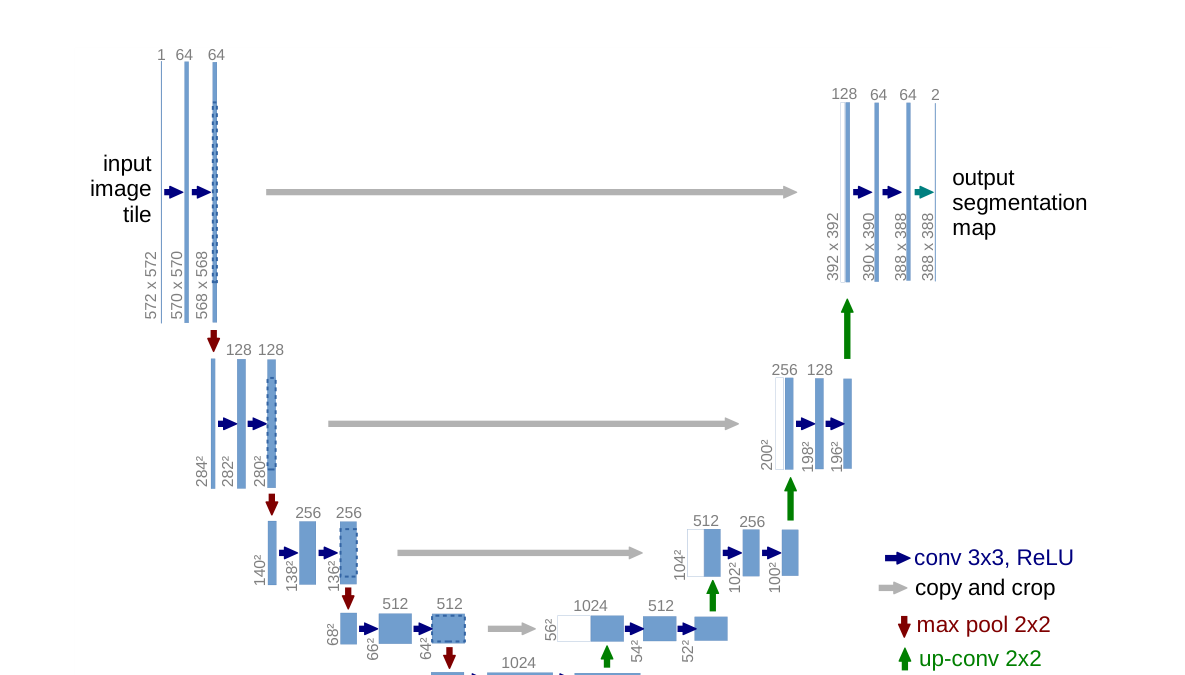
\includegraphics[width=0.98\textwidth]{unet-architecture.png}
  \caption{Original U-Net encoder--decoder structure. Source: Ronneberger et al.
  \cite{ronneberger2015unet}.}
  \label{fig:unet}
\end{figure}

\paragraph{Figure analysis.}
Figure~\ref{fig:unet} shows the main encoder--decoder idea. The left path reduces spatial
size and learns context. The right path restores resolution. Long skip connections move
detail to the decoder, which helps the model recover lesion boundaries.

The segmentation baseline is an Attention-Residual U-Net. Residual convolution blocks
support stable feature learning, while attention gates control skip features. Attention
gates were introduced to help U-Net focus on relevant regions \cite{oktay2018attention}.

\subsubsection{MCUNet-Seg}
MCUNet-Seg is the small segmentation model built for this project. Its encoder uses
MobileNetV2-style inverted residual blocks. An inverted residual first expands channels,
uses a depthwise convolution, and then projects features back to a narrow layer
\cite{sandler2018mobilenetv2}. Figure~\ref{fig:mobilenetv2} shows the main difference
from a standard residual block.

\fullpageimage{mobilenetv2-architecture.png}{Standard residual block and MobileNetV2
inverted residual block. Source: Sandler et al.
\cite{sandler2018mobilenetv2}.}{fig:mobilenetv2}

\paragraph{Figure analysis.}
Figure~\ref{fig:mobilenetv2} shows why the block is called inverted residual. The wide
feature space is inside the block, while the shortcut connects narrow bottlenecks. The
depthwise convolution reduces operation count and supports compact models.

The encoder design follows the compact-network principles introduced by MCUNet
\cite{lin2020mcunet}. MCUNet shows the value of small neural networks under strict
resource limits. This
thesis does not claim that MCUNet-Seg is an official MCUNet segmentation model. It is a
task-specific design with a U-Net-style decoder and four output channels. Its width
multiplier is 0.5.

\fullpageimage{project-architectures.png}{Implemented classifier and segmentation
architectures in this project.}{fig:project-architectures}

\paragraph{Figure analysis.}
Figure~\ref{fig:project-architectures} connects the literature blocks to the models that
were actually trained. The upper path adds the custom attention head after DenseNet-121.
The lower path uses small inverted-residual encoder stages and a compact decoder. This
figure describes the project implementation, not an unchanged published model.

\subsection{Training Policy}
All four experiments use seed 42 and the same fixed splits. AdamW is used because it
separates weight decay from the gradient update \cite{loshchilov2019adamw}. Mixed
precision supports faster numerical computation. The effective batch size is 16 through gradient
accumulation. Table~\ref{tab:training-config} gives the main settings.

\begin{table}[H]
\centering
\caption{Main training configuration.}
\label{tab:training-config}
\begin{tabularx}{\textwidth}{lXX}
\toprule
Setting & Classification & Segmentation\\
\midrule
Input size & 224$\times$224 & 256$\times$256\\
Batch / effective batch & 4 / 16 & 4 / 16\\
Maximum epochs & 35 & 100\\
Optimizer & AdamW & AdamW\\
Learning rate & $10^{-4}$ & $10^{-4}$\\
Weight decay & $10^{-4}$ & $10^{-4}$\\
Loss & weighted cross-entropy & 0.5 cross-entropy + 0.5 Dice\\
Early-stop patience & 8 epochs & 15 epochs\\
AMP & enabled & enabled\\
\bottomrule
\end{tabularx}
\end{table}

The DenseNet backbone is frozen for the first two epochs. Training stops when the main
validation metric does not improve for the configured patience. The best validation model,
not the last model, is loaded for test evaluation.

\subsection{Evaluation Metrics}
For classification, accuracy measures all correct samples. Precision for one class is
\begin{equation}
P=\frac{TP}{TP+FP}.
\end{equation}
Recall for one class is
\begin{equation}
R=\frac{TP}{TP+FN}.
\end{equation}
F1 is their harmonic mean:
\begin{equation}
F1=\frac{2PR}{P+R}.
\end{equation}
Macro F1 gives the same weight to every class. Weighted F1 uses class support. The report
also includes balanced accuracy, MCC, Cohen's kappa, ROC-AUC, average precision, log
loss, Brier score, and ten-bin ECE.

For segmentation, Dice is
\begin{equation}
Dice=\frac{2TP}{2TP+FP+FN}.
\end{equation}
IoU is
\begin{equation}
IoU=\frac{TP}{TP+FP+FN}.
\end{equation}
The disease macro values exclude background and give the same weight to each disease.
Boundary IoU measures edge agreement. Symmetric Hausdorff distance measures the largest
edge mismatch in pixels. A lower Hausdorff distance is better.

\subsection{Explainability}
Integrated Gradients compares the model output along a path from a baseline image to the
real image \cite{sundararajan2017integrated}. It gives one attribution value for each input
pixel. In this project, it is saved for qualitative inspection. It can show whether the
classifier looks at the leaf, but it cannot prove biological reasoning and is not used to
measure lesion area.

% =============================================================================
\subsection{Severity and Potential Yield Impact}

\subsubsection{Role in the Complete System}
Severity estimation is the bridge between image recognition and the potential yield-impact
scenario. Classification answers which disease is present. Segmentation answers where the
visible lesions are. Severity then answers how much of the leaf is affected. For this
reason, severity is treated as a separate main stage rather than a small post-processing
step.

The calculation uses two model outputs. The classifier provides the predicted disease
$d$, and the segmentation model provides the predicted lesion mask. A heuristic leaf mask
defines the area used as the denominator. The disease label and severity value are then
combined in the sensitivity model.

\subsubsection{Disease Severity Calculation}
Let $N_{lesion}$ be the number of predicted lesion pixels inside the leaf. Let $N_{leaf}$
be the number of pixels in the estimated leaf region. Severity is
\begin{equation}
S(\%)=100\times\frac{N_{lesion}}{N_{leaf}}.
\label{eq:severity}
\end{equation}
This area-ratio definition follows the standard interpretation of plant disease severity
as the proportion of visible plant area affected by symptoms \cite{bock2010severity}.
Only lesion pixels inside the estimated leaf region are counted. Background pixels outside
the leaf do not increase severity. If the predicted lesion contains several disease
channels, the channel selected for the predicted disease is used in the numerator.

The current leaf mask is not a manually reviewed ground truth. In several controlled
images, the heuristic includes most or all of the image. Therefore, $S$ is called a
heuristic-leaf severity proxy.

\subsubsection{Disease-Specific Potential Yield-Impact Calculation}
For disease $d$, the potential impact scenario is
\begin{equation}
I_d(\%)=\min\left(100,\,\beta_d S\right).
\label{eq:impact}
\end{equation}
where $d$ is the predicted disease, $S$ is severity in percent, and $\beta_d$ is the
disease-specific sensitivity factor. The three values of $\beta_d$ define low, central,
and high sensitivity scenarios. They are transparent analysis assumptions rather than
coefficients fitted from field measurements.
The minimum operation keeps the result at or below 100\%.

\subsubsection{Biological Evidence for Yield Impact}
The relationship between leaf symptoms and yield is supported by field-based plant
pathology, but it is not determined by image area alone. Iftikhar et al.~\cite{iftikhar2021tlcv}
studied TLCV in tomato cv.~Nagina during the 2017--2018 growing season. Their experiment
used four replications, recorded disease incidence at several times after planting, and
measured plant height, fruit number, fruit weight, and fruit yield. Incidence increased
from 8.32--25.00\% at 30 days after planting to 56.16--89.44\% at 75 days, depending on
planting date. The authors also reported that later planting was associated with more
whiteflies and higher incidence; the highest mean incidence in their planting-date
comparison was 60.06\%.

The same study reported a decrease in yield-related measurements across the planting-date
comparison. Mean fruit number ranged from 42 to 25.67 fruits per plant, fruit weight from
43 to 29 g, and yield from 3.47 to 2.01 kg per plant. The reported regression analysis
found a negative association between TLCV incidence and yield ($R^2=0.5483$), while the
association between whitefly population and yield was stronger ($R^2=0.9061$). The study
also reported a negative association between incidence and plant height
($R^2=0.8027$). These results show three important points for this project: disease
burden can affect several yield components, disease progress and environmental conditions
matter, and incidence is not identical to leaf-level severity.

They also explain why the present system does not stop after classification. The classifier
identifies the disease type, the segmenter estimates the visible affected area, and the
severity value provides the image-level variable used by the potential-impact calculation.

These values are evidence from a separate field study, not measurements from the present
image dataset. They therefore do not replace the disease-specific sensitivity scenarios in
Table~\ref{tab:beta}. Instead, they justify reporting severity and potential impact as
separate outputs and motivate future calibration with repeated images and measured harvest
records. The current project covers Early Blight, Late Blight, and Bacterial Spot, so the
TLCV findings are used as biological context rather than as a direct coefficient for any
of the three supported diseases. For the supported diseases, previous studies have also
reported yield or quality effects: Early Blight is associated with measurable yield loss
\cite{saha2012earlyblight}, Late Blight losses vary with epidemic conditions and cultivar
\cite{fontem2003blights,nowicki2012lateblight}, and Bacterial Spot can reduce fresh-market
yield and quality \cite{pohronezny1983bacterialspot}. These references support the use of
the predicted class $d$ in Equation~\ref{eq:impact}; the lesion literature supports the use
of $S$; and the TLCV study supports the broader biological link between disease burden and
crop-level effects. None of these studies supplies a calibrated coefficient for the
present PlantVillage-based image split.

\begin{table}[H]
\centering
\caption{Sensitivity assumptions for potential yield impact.}
\label{tab:beta}
\begin{tabular}{lrrr}
\toprule
Disease & $\beta_{low}$ & $\beta_{central}$ & $\beta_{high}$\\
\midrule
Early Blight & 0.50 & 0.60 & 0.70\\
Late Blight & 1.00 & 1.10 & 1.20\\
Bacterial Spot & 0.30 & 0.40 & 0.45\\
\bottomrule
\end{tabular}
\end{table}

\noindent\textit{Basis of the assumptions:} published studies report yield effects for
Early Blight \cite{saha2012earlyblight}, Late Blight
\cite{fontem2003blights,nowicki2012lateblight}, and Bacterial Spot
\cite{pohronezny1983bacterialspot}. The scenario coefficients in
Table~\ref{tab:beta} are not presented as values measured by those studies.

The literature confirms that these diseases can reduce yield, but it does not validate one
universal percentage slope for this image dataset. Early Blight studies report an absolute
yield slope in tonnes per hectare \cite{saha2012earlyblight}. Late Blight loss changes with
variety and epidemic conditions \cite{fontem2003blights,nowicki2012lateblight}. Bacterial
Spot can reduce marketable yield and quality \cite{pohronezny1983bacterialspot}. The beta
values are therefore project scenarios, not fitted causal coefficients.

\subsubsection{Worked Calculation Example}
Assume that a leaf mask contains 65,536 pixels and the model predicts 6,554 disease pixels
inside it. Using Equation~\ref{eq:severity}, the severity is
\begin{equation}
S=100\times\frac{6{,}554}{65{,}536}\approx 10.0\%.
\end{equation}
If the classifier predicts Early Blight, the low, central, and high scenarios are
$0.50\times10=5.0\%$, $0.60\times10=6.0\%$, and
$0.70\times10=7.0\%$. For the same severity, Late Blight gives 10.0\%, 11.0\%, and
12.0\%, while Bacterial Spot gives 3.0\%, 4.0\%, and 4.5\%. This example shows why both
the segmented area and the disease class are required.

\subsubsection{Interpretation and Scientific Limit}
The output describes a potential sensitivity scenario for one image. It does not directly
predict harvested tomato weight. Real yield also depends on the plant growth stage,
cultivar, weather, treatment, disease progress, and the number of affected leaves. Paired
field measurements are required before the sensitivity factors can be fitted as validated
yield-loss coefficients.

% =============================================================================
\section{Result}

\subsection{Experiment Completion}
All four experiments completed successfully and were evaluated using their best
validation states.

Early stopping worked as planned. The classification baseline selected epoch 12 and
stopped at epoch 20. The attention classifier selected epoch 8 and stopped at epoch 16.
The segmentation baseline selected epoch 31 and stopped at epoch 46. MCUNet-Seg
selected epoch 52 and stopped at epoch 67.

\subsection{Classification Results}

\subsubsection{Aggregate comparison}
Table~\ref{tab:classification-results} compares the two classifiers on the same 662-image
test split. The plain DenseNet-121 baseline gave the best result. The custom attention
head did not improve accuracy.

\begin{table}[H]
\centering
\caption{Held-out classification results.}
\label{tab:classification-results}
\small
\resizebox{\textwidth}{!}{%
\begin{tabular}{lrrrrrr}
\toprule
Model & Accuracy & Macro F1 & Bal. Acc. & MCC & ROC-AUC & ECE\\
\midrule
DenseNet-121 baseline & 1.0000 & 1.0000 & 1.0000 & 1.0000 & 1.0000 & 0.0058\\
DenseNet + attention & 0.9909 & 0.9895 & 0.9925 & 0.9877 & 1.0000 & 0.0067\\
\bottomrule
\end{tabular}
}
\end{table}

The baseline correctly classified all 662 test images. Its test log loss was 0.0062 and its
multiclass Brier score was 0.0014. The attention classifier made six errors. Its log loss
was 0.0177 and its Brier score was 0.0105.

\begin{figure}[H]
  \centering
  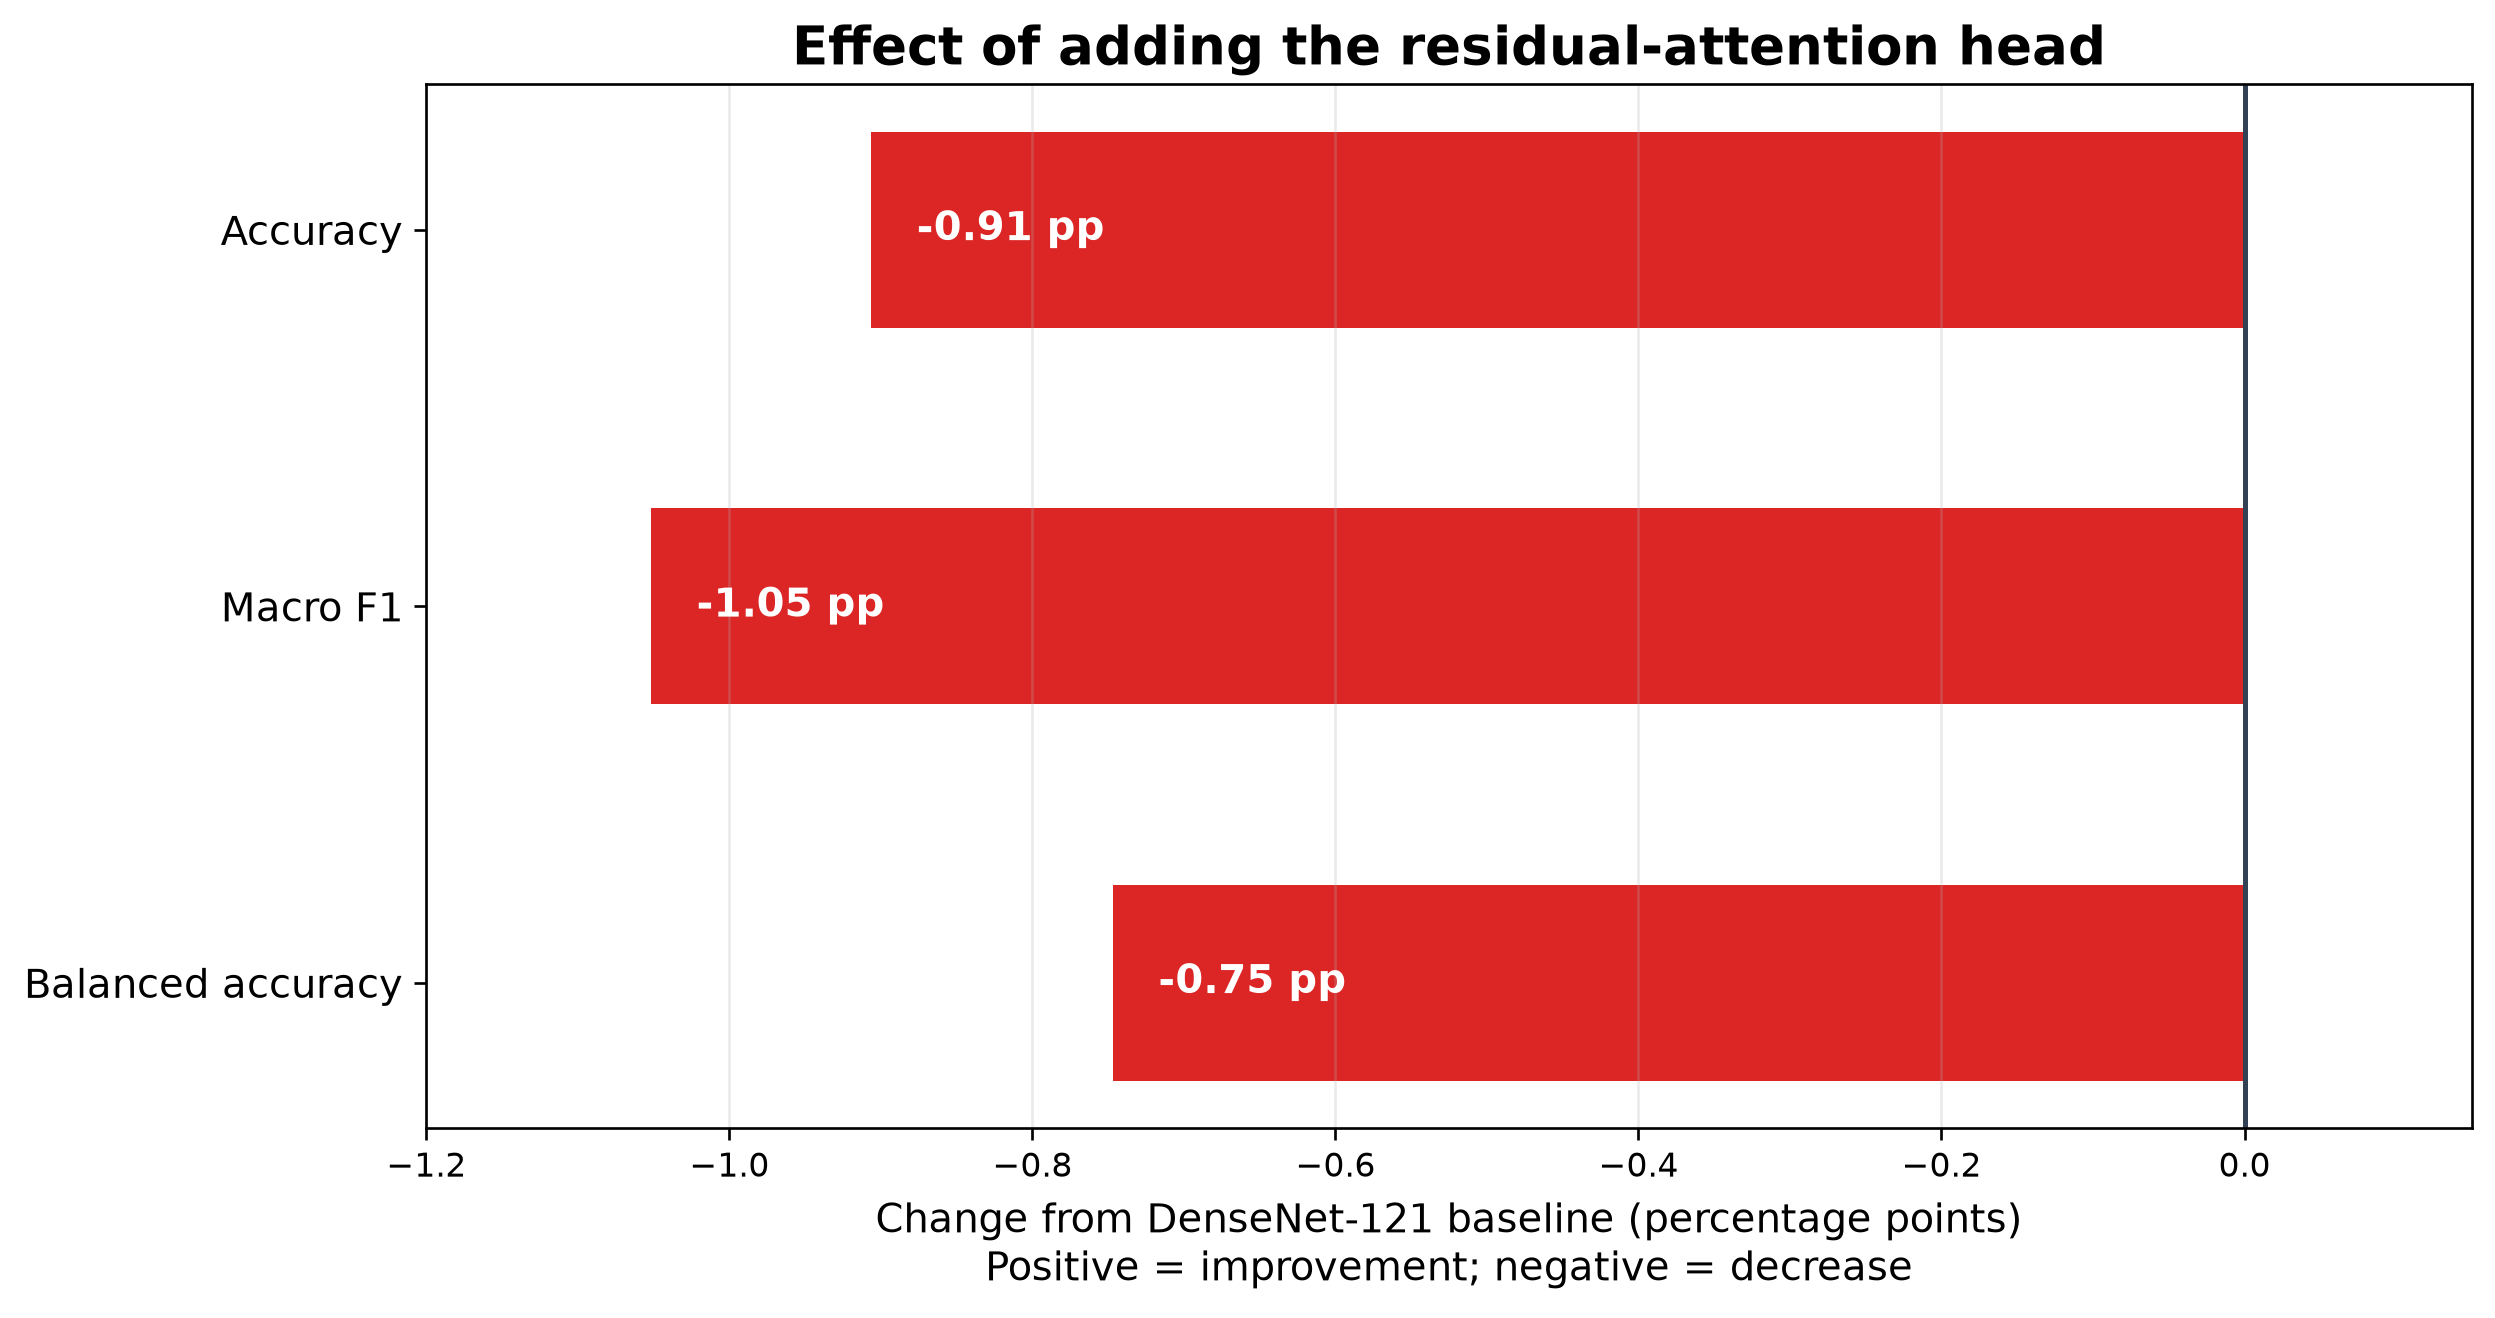
\includegraphics[width=0.98\textwidth]{classification-ablation.png}
  \caption{Change in classification score after adding the residual-attention head. A
  negative value means that the custom model performs worse than the plain baseline.}
  \label{fig:classification-ablation}
\end{figure}

\paragraph{Figure analysis.}
Figure~\ref{fig:classification-ablation} is an ablation result. Its purpose is to test
whether the extra residual-attention head improves DenseNet-121. All three bars are below
zero, so the custom head reduces accuracy, macro F1, and balanced accuracy. The graph
reports the change in percentage points; it does not hide or rescale the original scores.

\subsubsection{Interpretation of the High Classification Scores}
PlantVillage images use controlled backgrounds and clear disease examples. This makes the
held-out split easier than real field photography. Exact duplicates were removed and image
groups were kept inside one split, but these controls cannot remove the domain gap. The
near-perfect result should therefore be read as performance on this controlled dataset,
not as proof of near-perfect diagnosis in farms. An external field-image test is required.

\subsubsection{Per-class performance}
The attention classifier kept perfect recall for healthy and Early Blight. Three Late
Blight samples and three Bacterial Spot samples were incorrect. Five of these six errors
were predicted as Early Blight.

\begin{table}[H]
\centering
\caption{Per-class metrics for DenseNet-121 with the custom attention head.}
\label{tab:classification-per-class}
\begin{tabular}{lrrrrr}
\toprule
Class & Precision & Recall & F1 & TP & FP/FN\\
\midrule
Healthy & 1.0000 & 1.0000 & 1.0000 & 159 & 0 / 0\\
Early Blight & 0.9524 & 1.0000 & 0.9756 & 100 & 5 / 0\\
Late Blight & 0.9947 & 0.9842 & 0.9894 & 187 & 1 / 3\\
Bacterial Spot & 1.0000 & 0.9859 & 0.9929 & 210 & 0 / 3\\
\bottomrule
\end{tabular}
\end{table}

\fullpageimage{classification-training-curves.png}{Training and validation curves for
the custom residual-attention classifier.}{fig:classification-training}

\paragraph{Figure analysis.}
Figure~\ref{fig:classification-training} shows fast learning after the frozen-backbone
period. Validation performance becomes very high after only a few epochs. The later
changes are small, so early stopping avoids unnecessary training after the best epoch.

\begin{figure}[H]
  \centering
  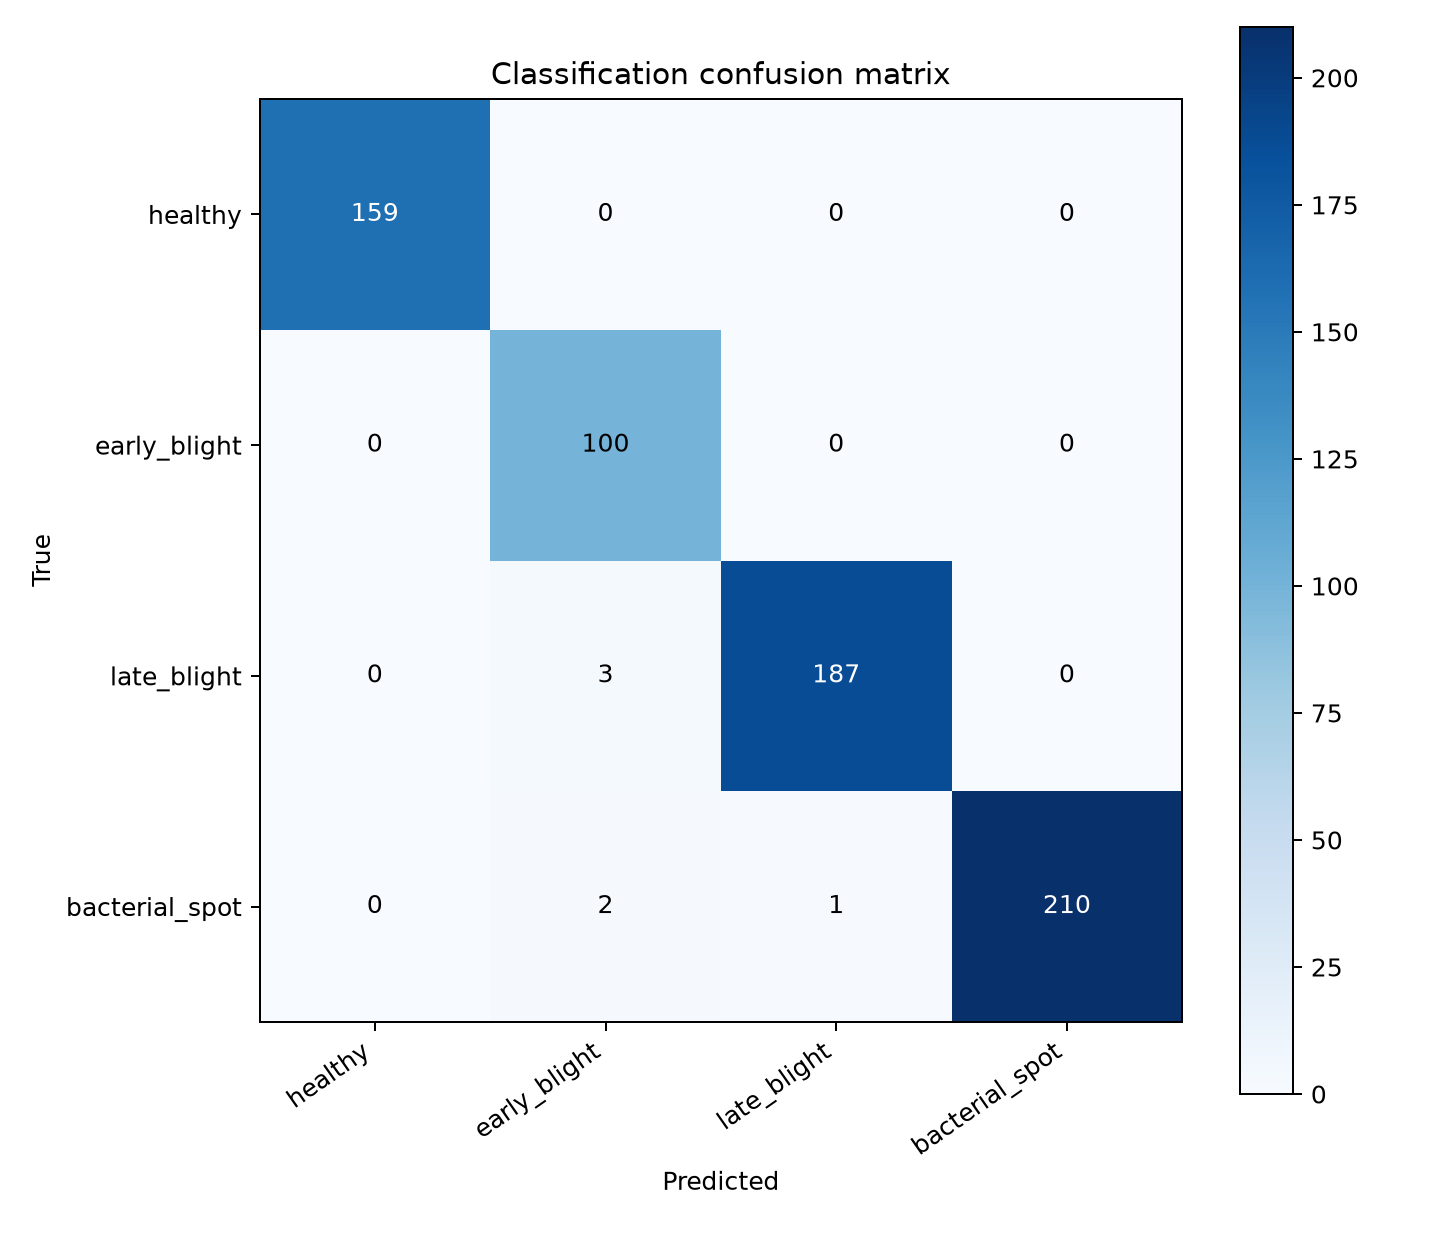
\includegraphics[width=0.98\textwidth]{classification-confusion-matrix.png}
  \caption{Test confusion matrix for the custom residual-attention classifier.}
  \label{fig:classification-confusion}
\end{figure}

\paragraph{Figure analysis.}
Figure~\ref{fig:classification-confusion} shows only six errors. The errors are not spread
equally: Early Blight receives five false positives from the other disease classes. Healthy
images are all classified correctly.

\fullpageimage{classification-roc-pr-calibration.png}{One-versus-rest ROC,
precision--recall, and confidence calibration plots.}{fig:classification-curves}

\paragraph{Figure analysis.}
Figure~\ref{fig:classification-curves} shows near-perfect ranking for every one-versus-rest
class. The calibration panel is also close to the ideal diagonal. These plots support the
high test scores, but they still describe the controlled domain only.

The very high scores must be read with care. PlantVillage images often use controlled
backgrounds. The data gate removed exact duplicates and kept UUID variants in one split,
but a perfect controlled test score does not prove perfect field performance.

\subsection{Segmentation Results}

\subsubsection{Aggregate comparison}
The Attention-Residual U-Net clearly outperformed MCUNet-Seg. It improved disease macro
Dice by 0.2102 and macro IoU by 0.2172. It also had much better boundary agreement.

\begin{table}[H]
\centering
\caption{Held-out segmentation results. Disease macro values exclude background.}
\label{tab:segmentation-results}
\small
\resizebox{\textwidth}{!}{%
\begin{tabular}{lrrrrrr}
\toprule
Model & Dice & IoU & Precision & Recall & Boundary IoU & Pixel Acc.\\
\midrule
Attention-Residual U-Net & 0.7346 & 0.5855 & 0.8204 & 0.6789 & 0.2421 & 0.9405\\
MCUNet-Seg & 0.5244 & 0.3683 & 0.5976 & 0.5275 & 0.0917 & 0.9073\\
\bottomrule
\end{tabular}
}
\end{table}

\begin{figure}[H]
  \centering
  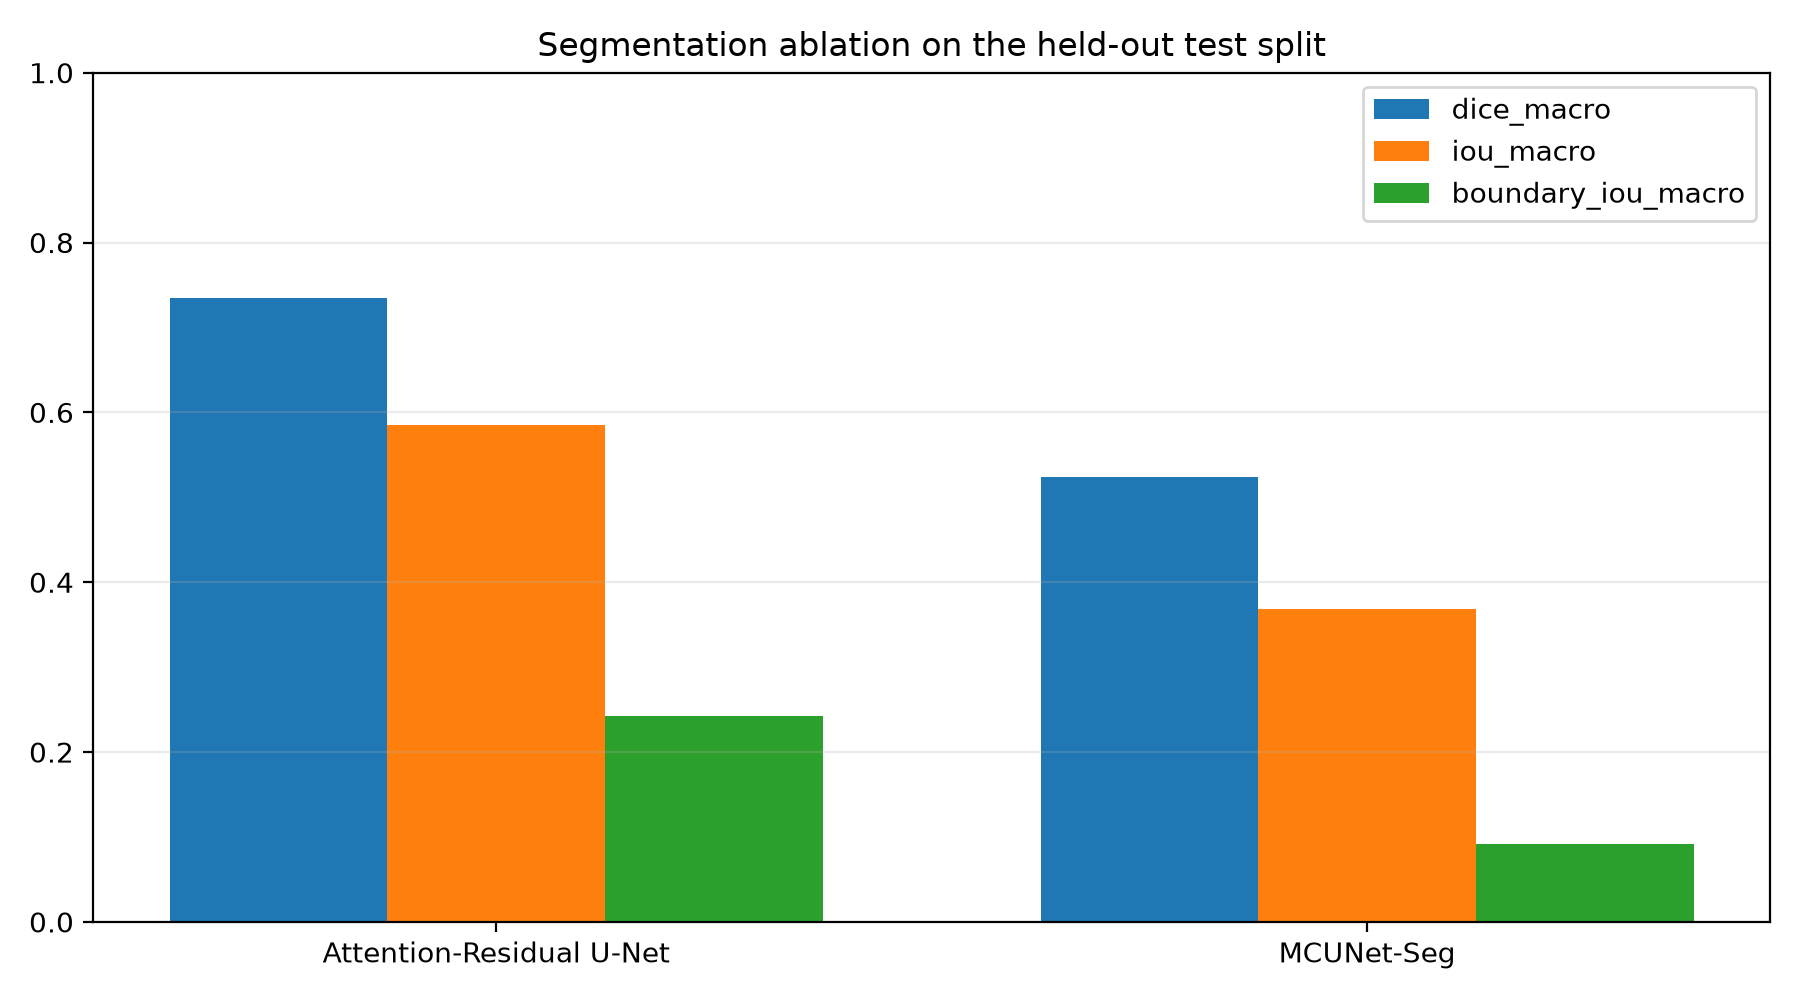
\includegraphics[width=0.98\textwidth]{segmentation-ablation.png}
  \caption{Segmentation ablation on the fixed 68-image test split.}
  \label{fig:segmentation-ablation}
\end{figure}

\paragraph{Figure analysis.}
Figure~\ref{fig:segmentation-ablation} shows a large and consistent baseline advantage.
The gap is visible in Dice, IoU, and boundary IoU, so it is not caused by only one metric.
MCUNet-Seg is smaller, but the accuracy cost is clear.

\subsubsection{Disease-level results}
Late Blight was the strongest class for both models. Early Blight was the hardest class,
especially for MCUNet-Seg. Its Early Blight recall was only 0.2141, so many lesion pixels
were missed.

\begin{table}[H]
\centering
\caption{Disease-level Dice and IoU on the segmentation test split.}
\label{tab:segmentation-per-class}
\begin{tabular}{llrrrr}
\toprule
Model & Disease & Precision & Recall & Dice & IoU\\
\midrule
Attention-Residual U-Net & Early Blight & 0.8577 & 0.5132 & 0.6421 & 0.4729\\
 & Late Blight & 0.8178 & 0.8152 & 0.8165 & 0.6899\\
 & Bacterial Spot & 0.7858 & 0.7084 & 0.7451 & 0.5937\\
\midrule
MCUNet-Seg & Early Blight & 0.6038 & 0.2141 & 0.3161 & 0.1877\\
 & Late Blight & 0.5505 & 0.7841 & 0.6469 & 0.4780\\
 & Bacterial Spot & 0.6386 & 0.5843 & 0.6102 & 0.4391\\
\bottomrule
\end{tabular}
\end{table}

\fullpageimage{segmentation-baseline-curves.png}{Training and validation curves for the
Attention-Residual U-Net.}{fig:segmentation-baseline-curves}

\paragraph{Figure analysis.}
Figure~\ref{fig:segmentation-baseline-curves} shows strong improvement during the first
part of training, followed by variation around a plateau. The best validation Dice is kept
at epoch 31 instead of using the lower-scoring final epoch.

\fullpageimage{mcunet-training-curves.png}{Training and validation curves for
MCUNet-Seg.}{fig:mcunet-training-curves}

\paragraph{Figure analysis.}
Figure~\ref{fig:mcunet-training-curves} shows slower learning and a lower plateau than the
baseline. The best validation Dice appears at epoch 52. Later epochs do not give a stable
improvement, so early stopping selects the best checkpoint.

\subsubsection{Qualitative comparison}
Figures~\ref{fig:baseline-bacterial}--\ref{fig:mcunet-early} show the same three test
disease types for both models. Each large figure contains the input, ground truth,
prediction, and a prediction overlay. The baseline often follows the main lesion better.
Both models can miss small separated spots.

\begin{figure}[H]
  \centering
  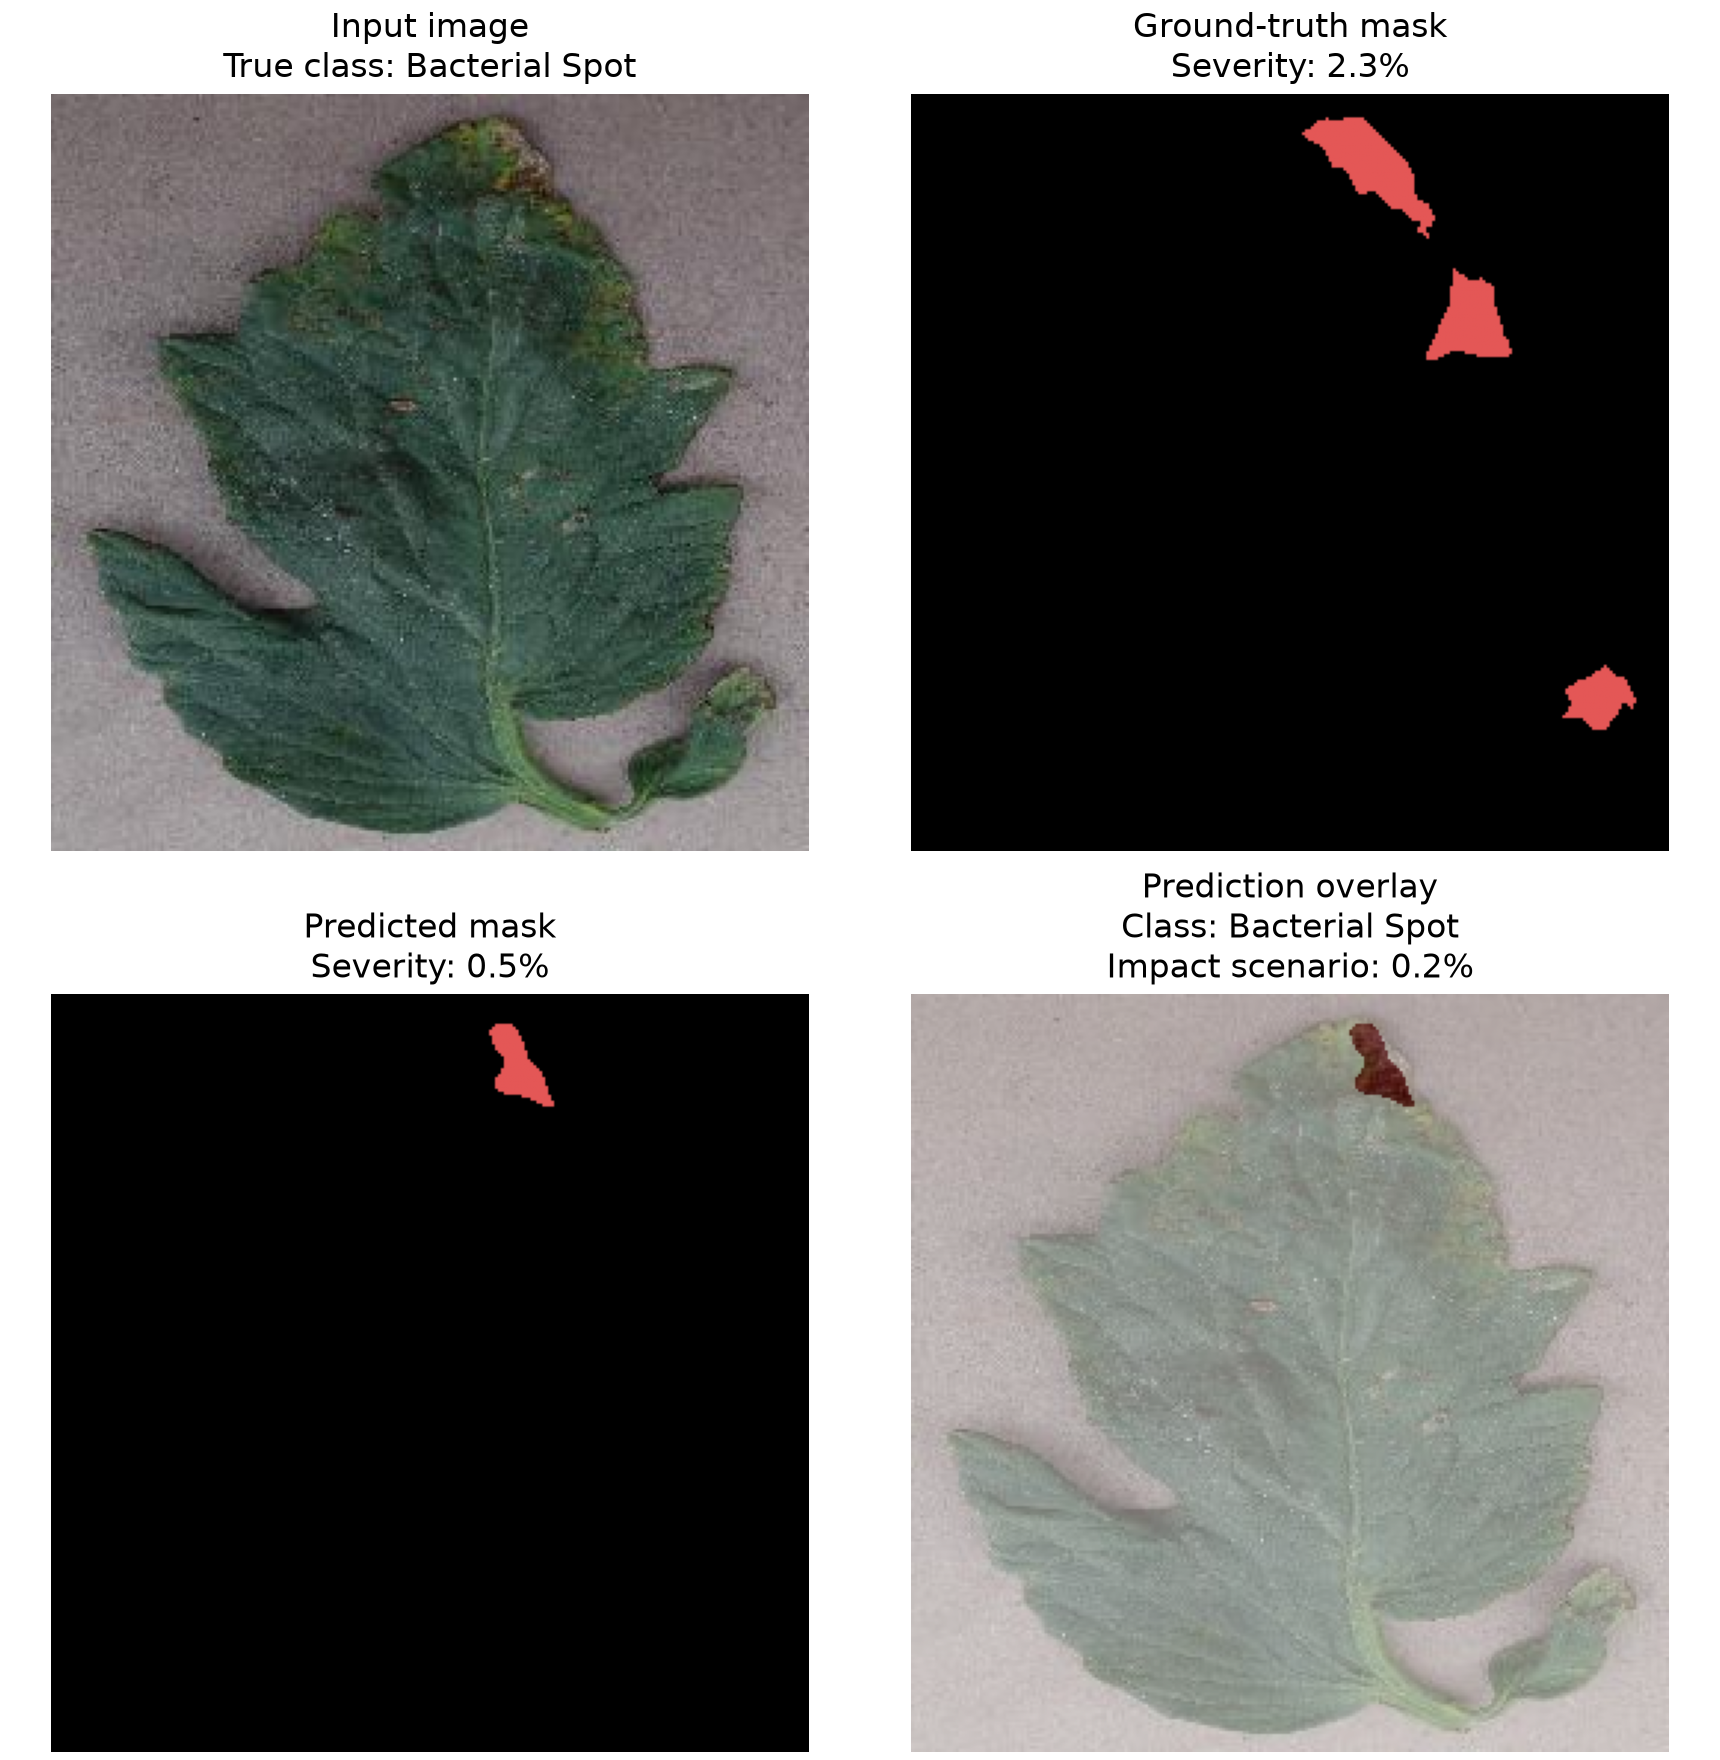
\includegraphics[width=0.94\textwidth]{baseline-bacterial.png}
  \caption{Attention-Residual U-Net prediction for a Bacterial Spot sample.}
  \label{fig:baseline-bacterial}
\end{figure}

\paragraph{Figure analysis.}
Figure~\ref{fig:baseline-bacterial} shows that the baseline identifies important parts of
the Bacterial Spot lesions. Some small separated spots are still missed, which can reduce
the predicted severity.

\begin{figure}[H]
  \centering
  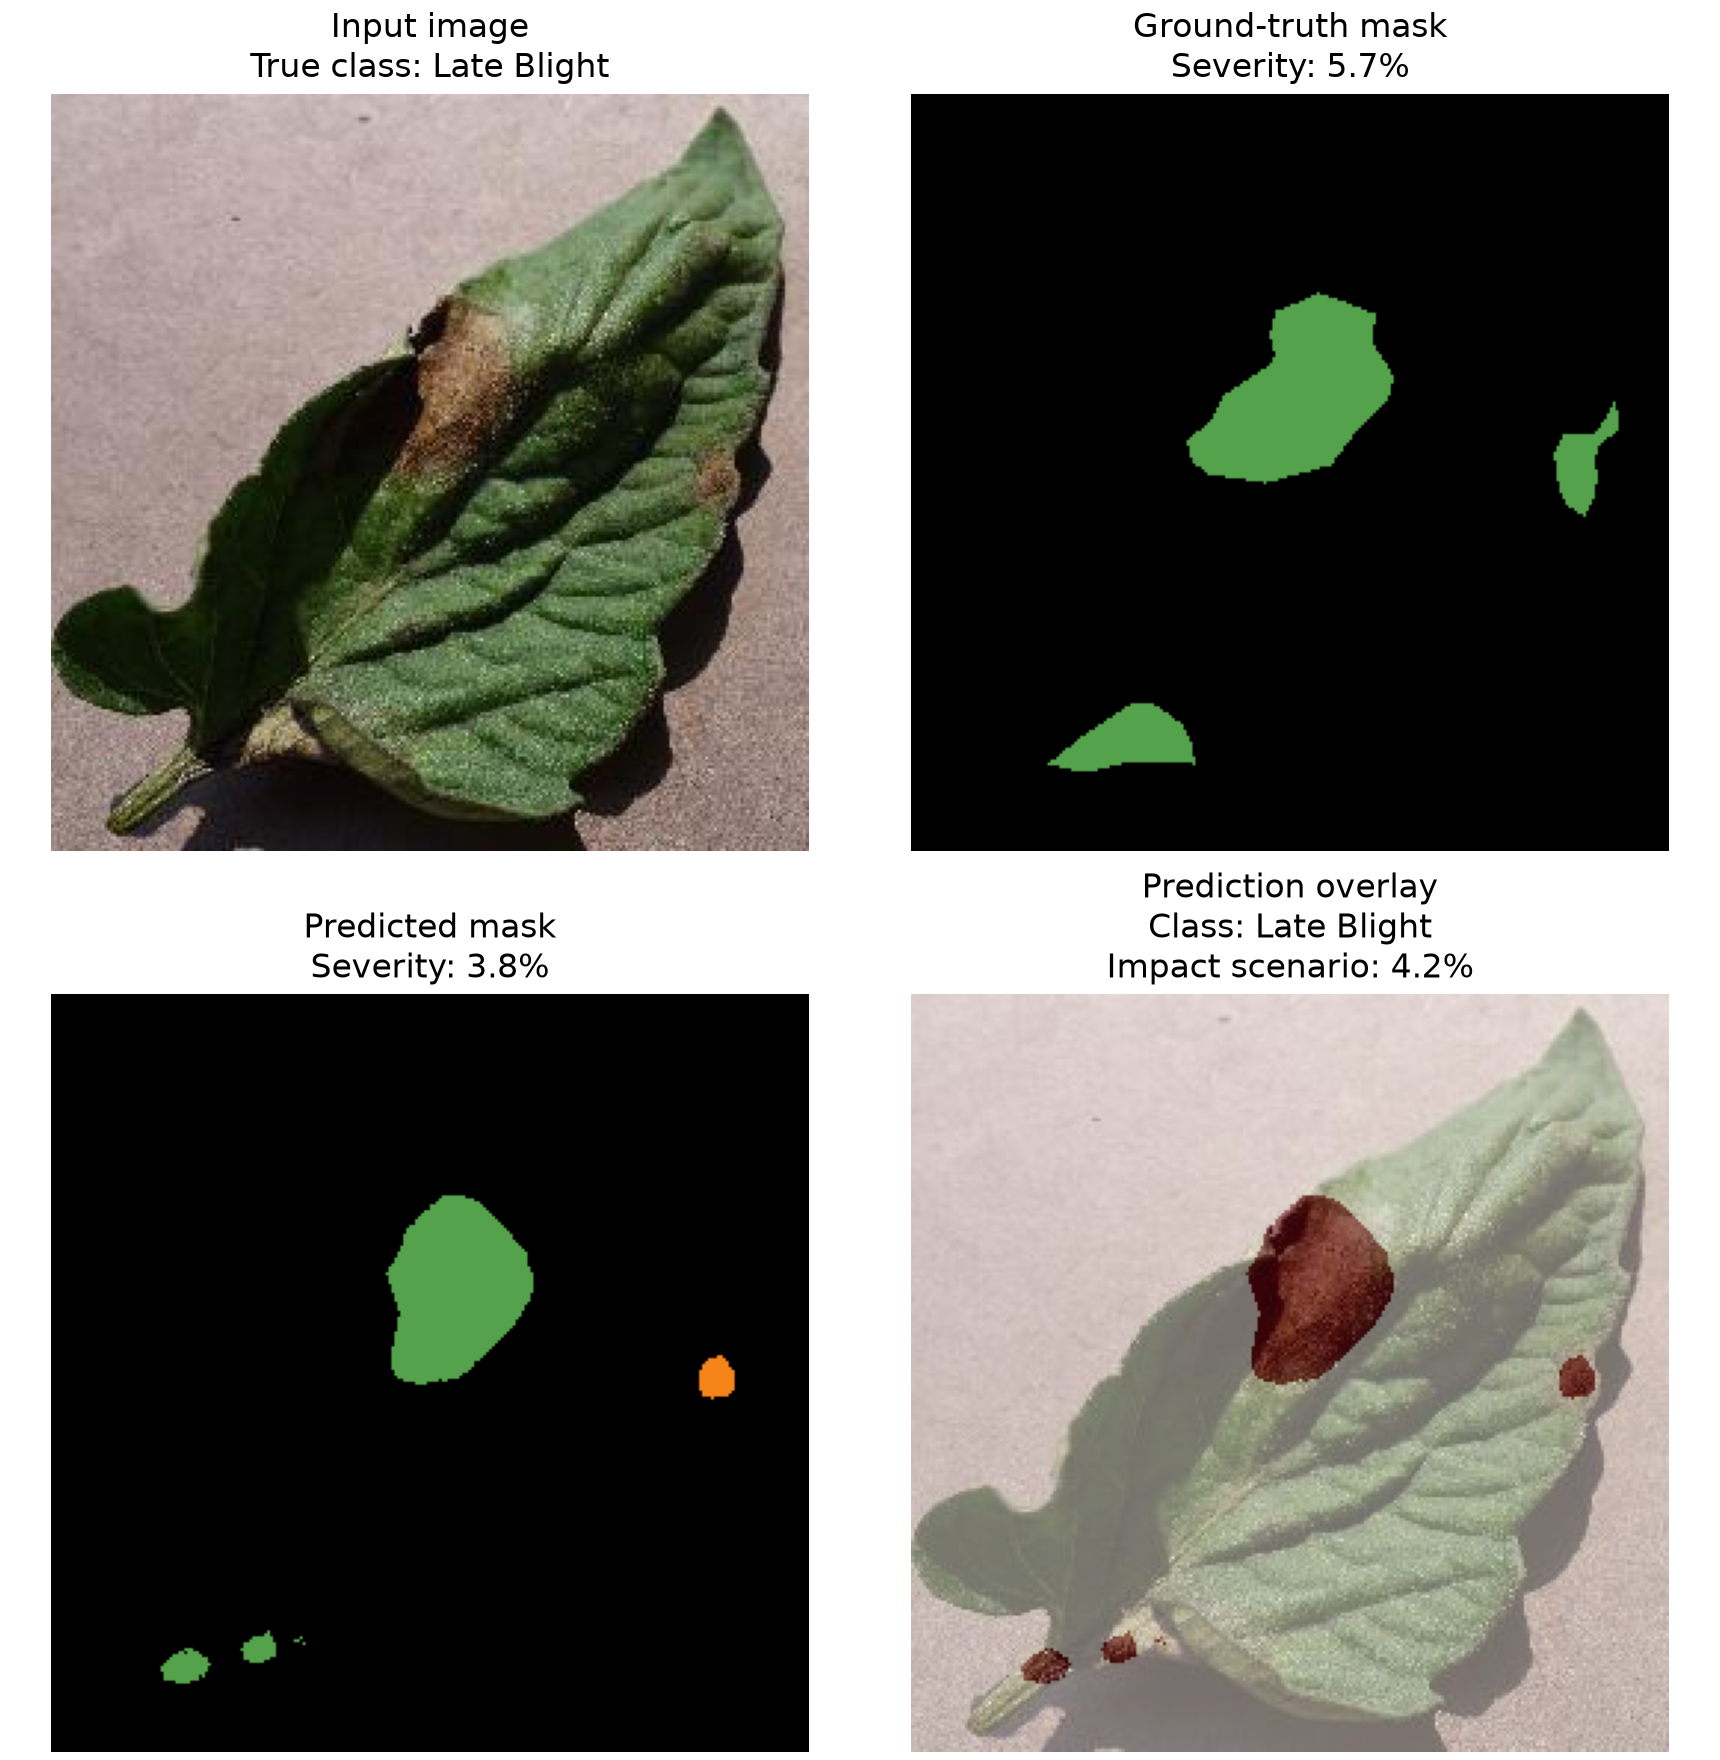
\includegraphics[width=0.94\textwidth]{baseline-late.png}
  \caption{Attention-Residual U-Net prediction for a Late Blight sample.}
  \label{fig:baseline-late}
\end{figure}

\paragraph{Figure analysis.}
Figure~\ref{fig:baseline-late} shows good agreement for the main Late Blight region. The
predicted mask follows the large lesion more closely than the small-model result shown
later.

\begin{figure}[H]
  \centering
  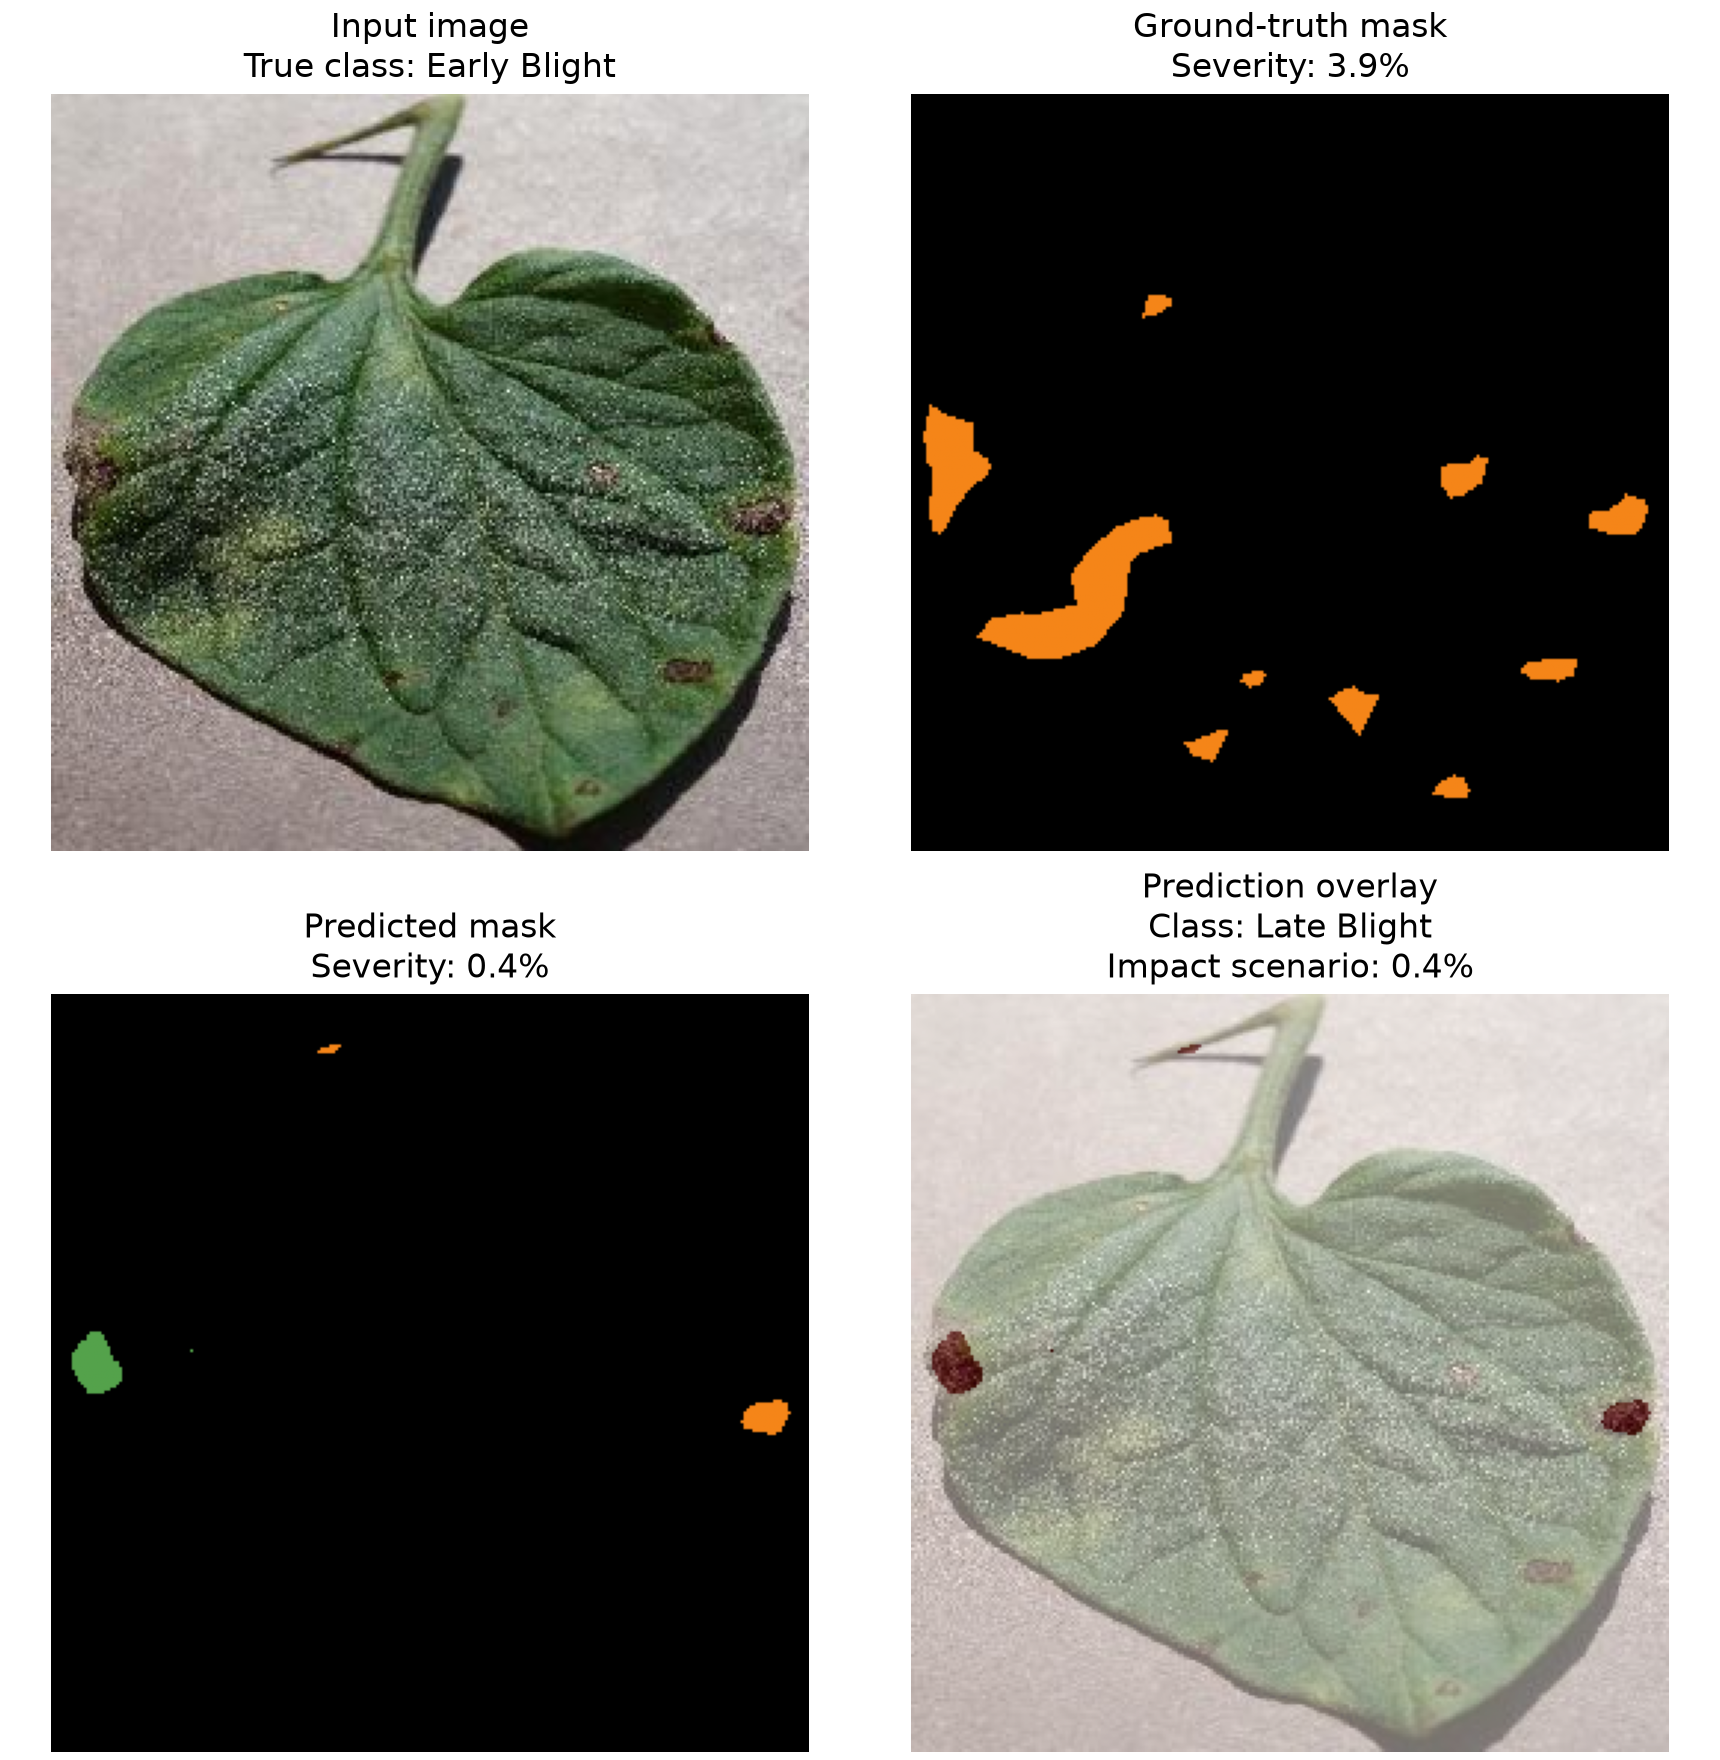
\includegraphics[width=0.94\textwidth]{baseline-early.png}
  \caption{Attention-Residual U-Net prediction for an Early Blight sample.}
  \label{fig:baseline-early}
\end{figure}

\paragraph{Figure analysis.}
Figure~\ref{fig:baseline-early} shows that Early Blight remains difficult because many
spots are small and separated. Missing these small regions explains the lower Early Blight
recall and the underestimation of severity.

\begin{figure}[H]
  \centering
  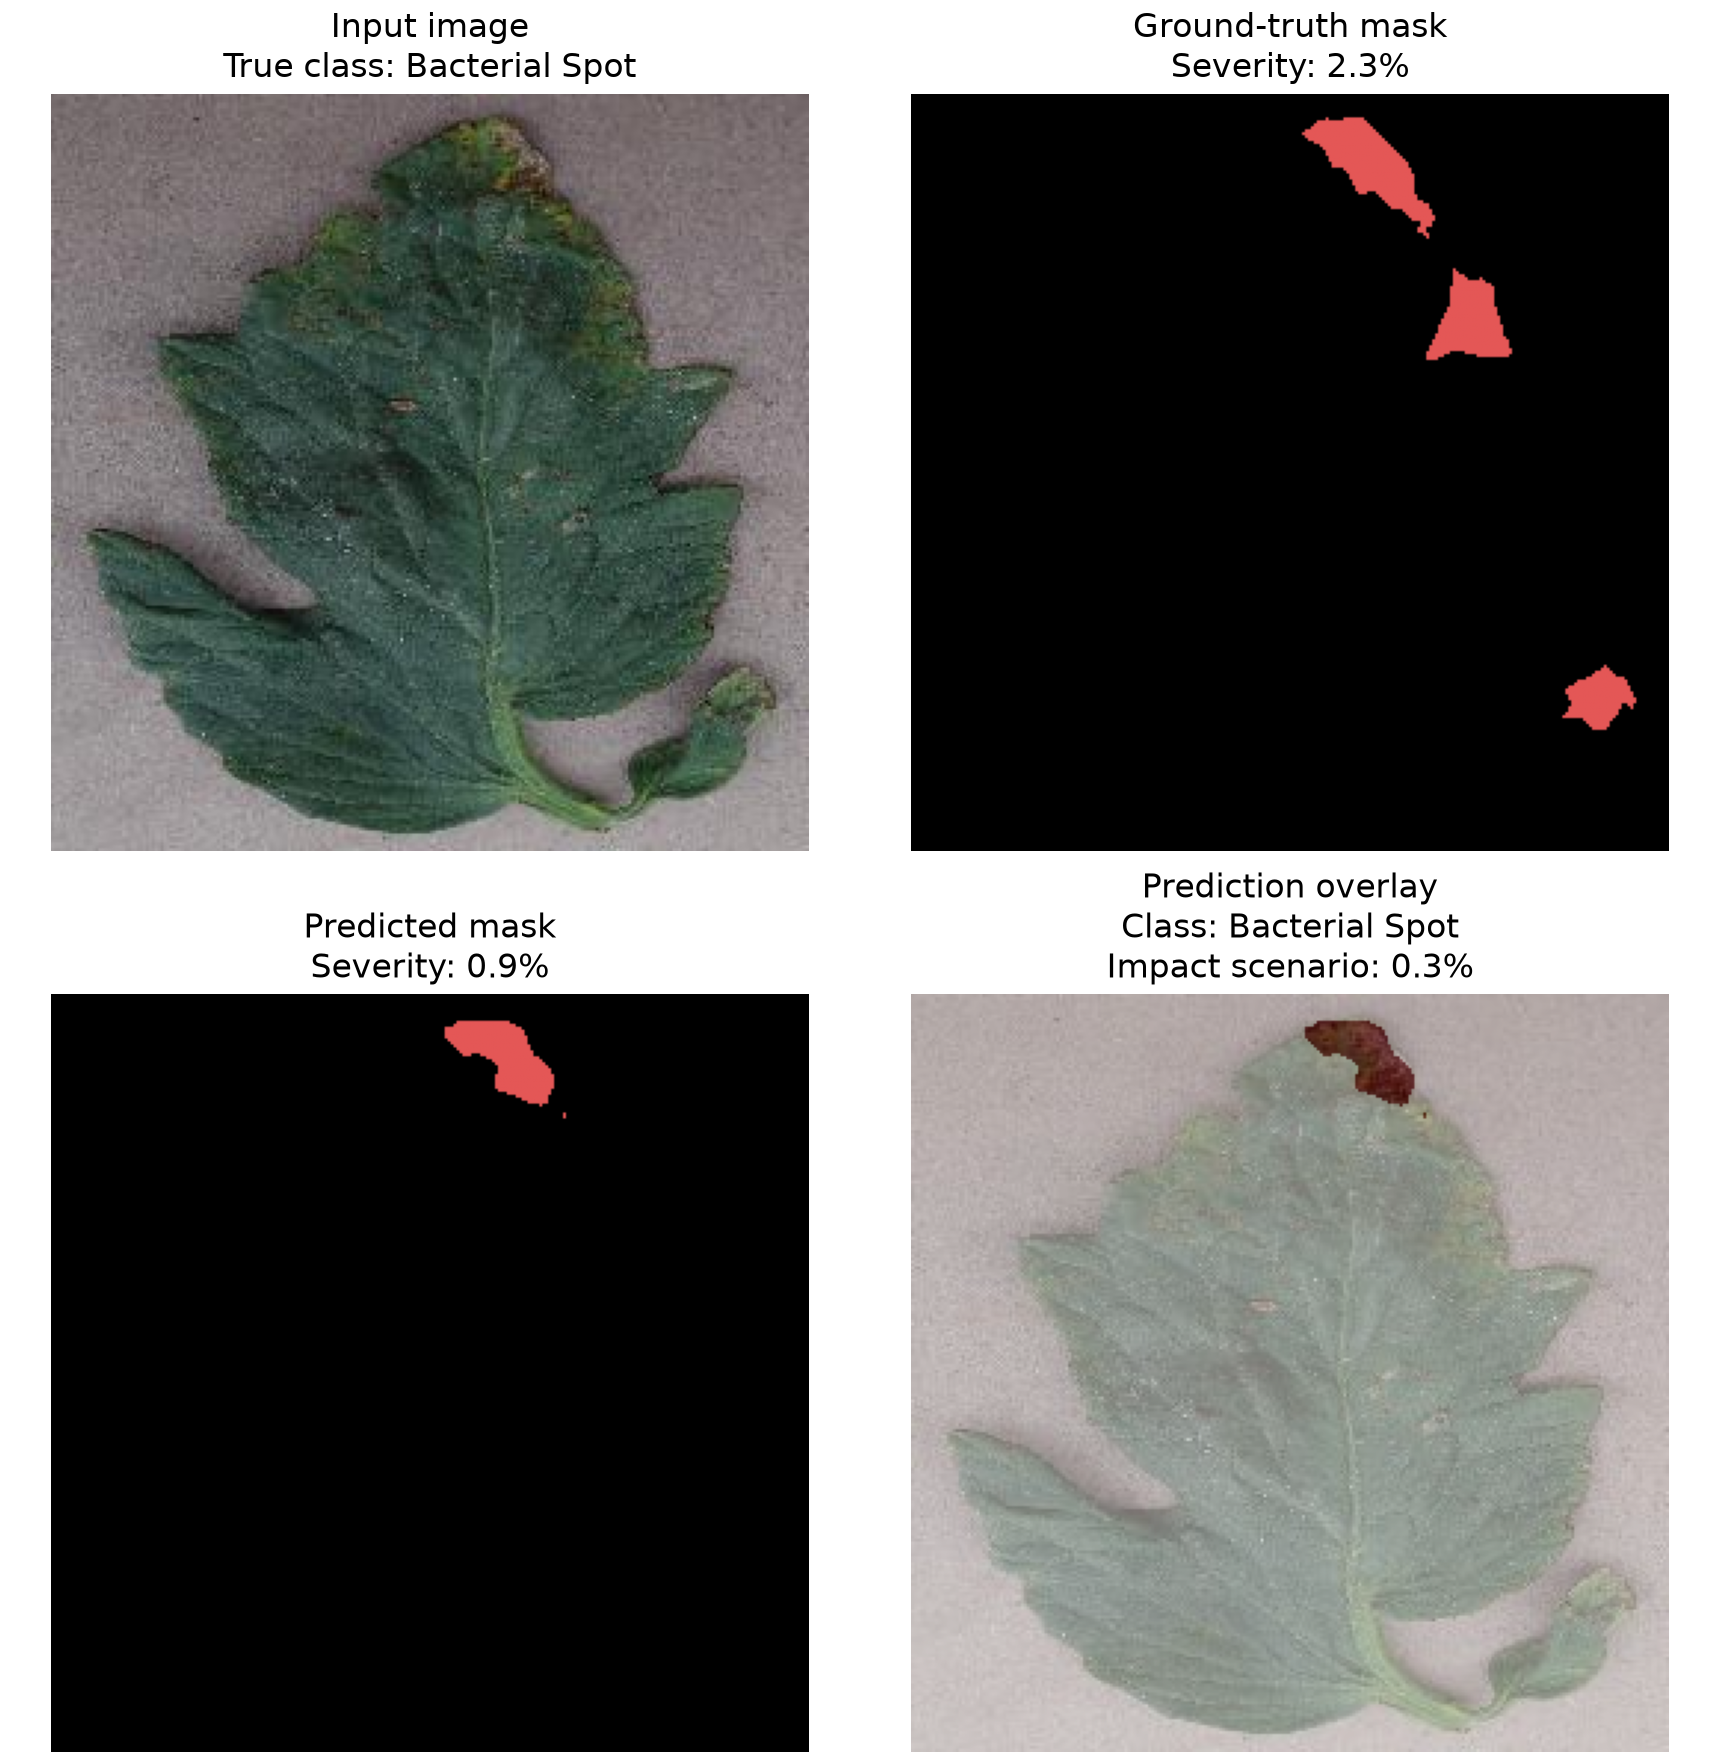
\includegraphics[width=0.94\textwidth]{mcunet-bacterial.png}
  \caption{MCUNet-Seg prediction for a Bacterial Spot sample.}
  \label{fig:mcunet-bacterial}
\end{figure}

\paragraph{Figure analysis.}
Figure~\ref{fig:mcunet-bacterial} shows that MCUNet-Seg finds part of the lesion but
does not recover all small regions. This is consistent with its lower Bacterial Spot Dice
score compared with the baseline.

\begin{figure}[H]
  \centering
  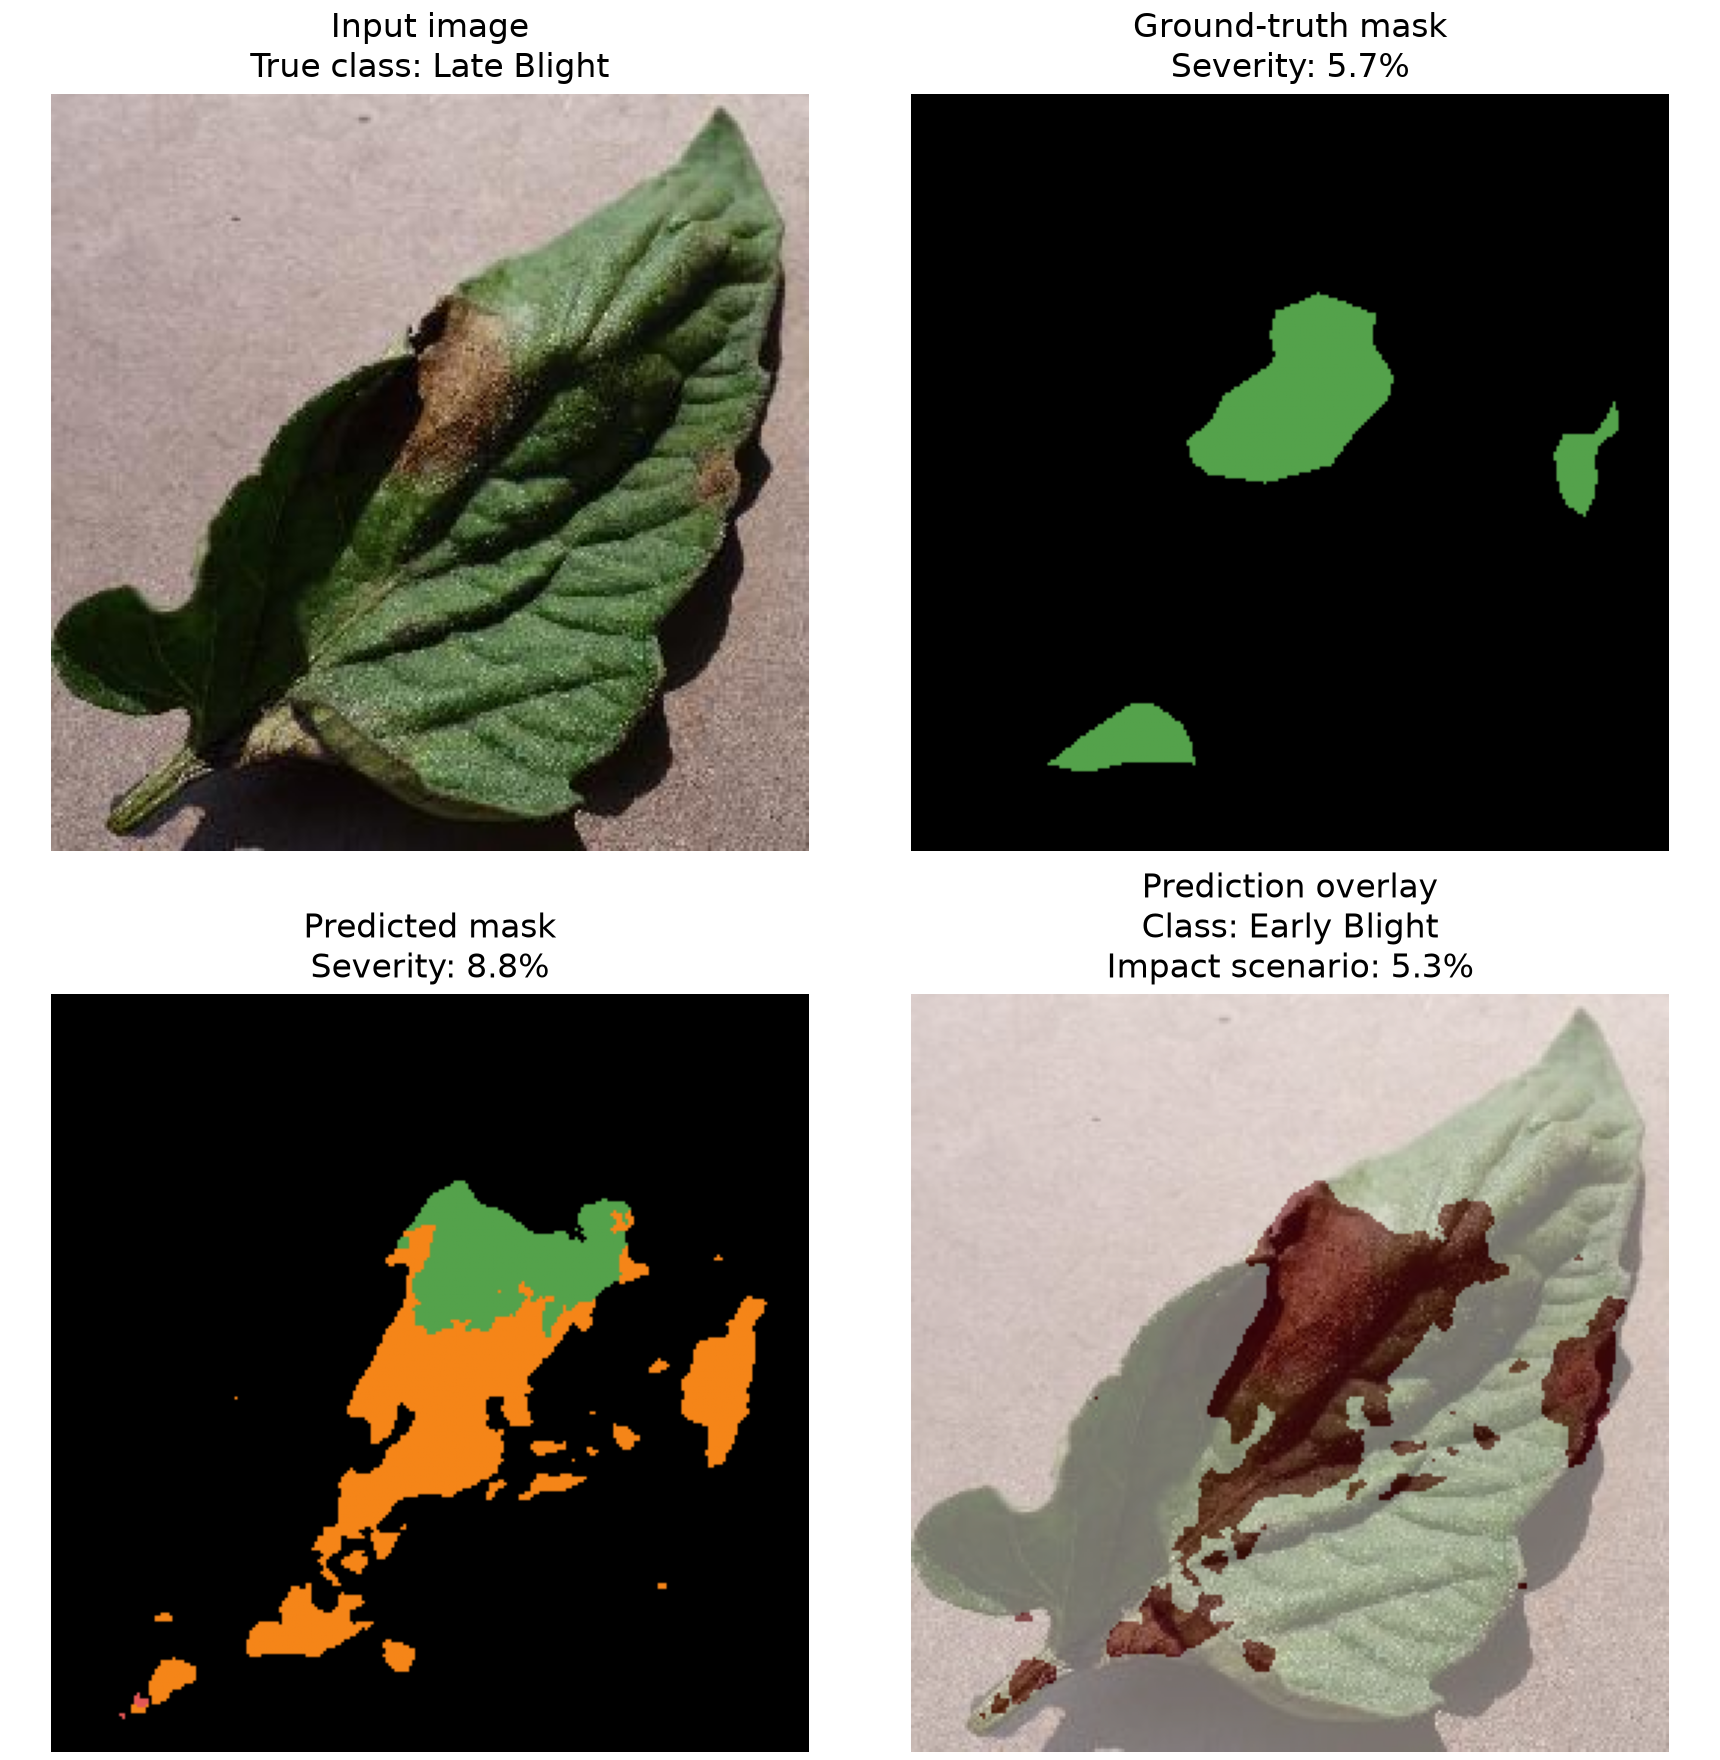
\includegraphics[width=0.94\textwidth]{mcunet-late.png}
  \caption{MCUNet-Seg prediction for a Late Blight sample.}
  \label{fig:mcunet-late}
\end{figure}

\paragraph{Figure analysis.}
Figure~\ref{fig:mcunet-late} shows extra pixels from another disease channel inside the
large lesion. This class confusion lowers precision and boundary agreement even when the
main damaged area is detected.

\begin{figure}[H]
  \centering
  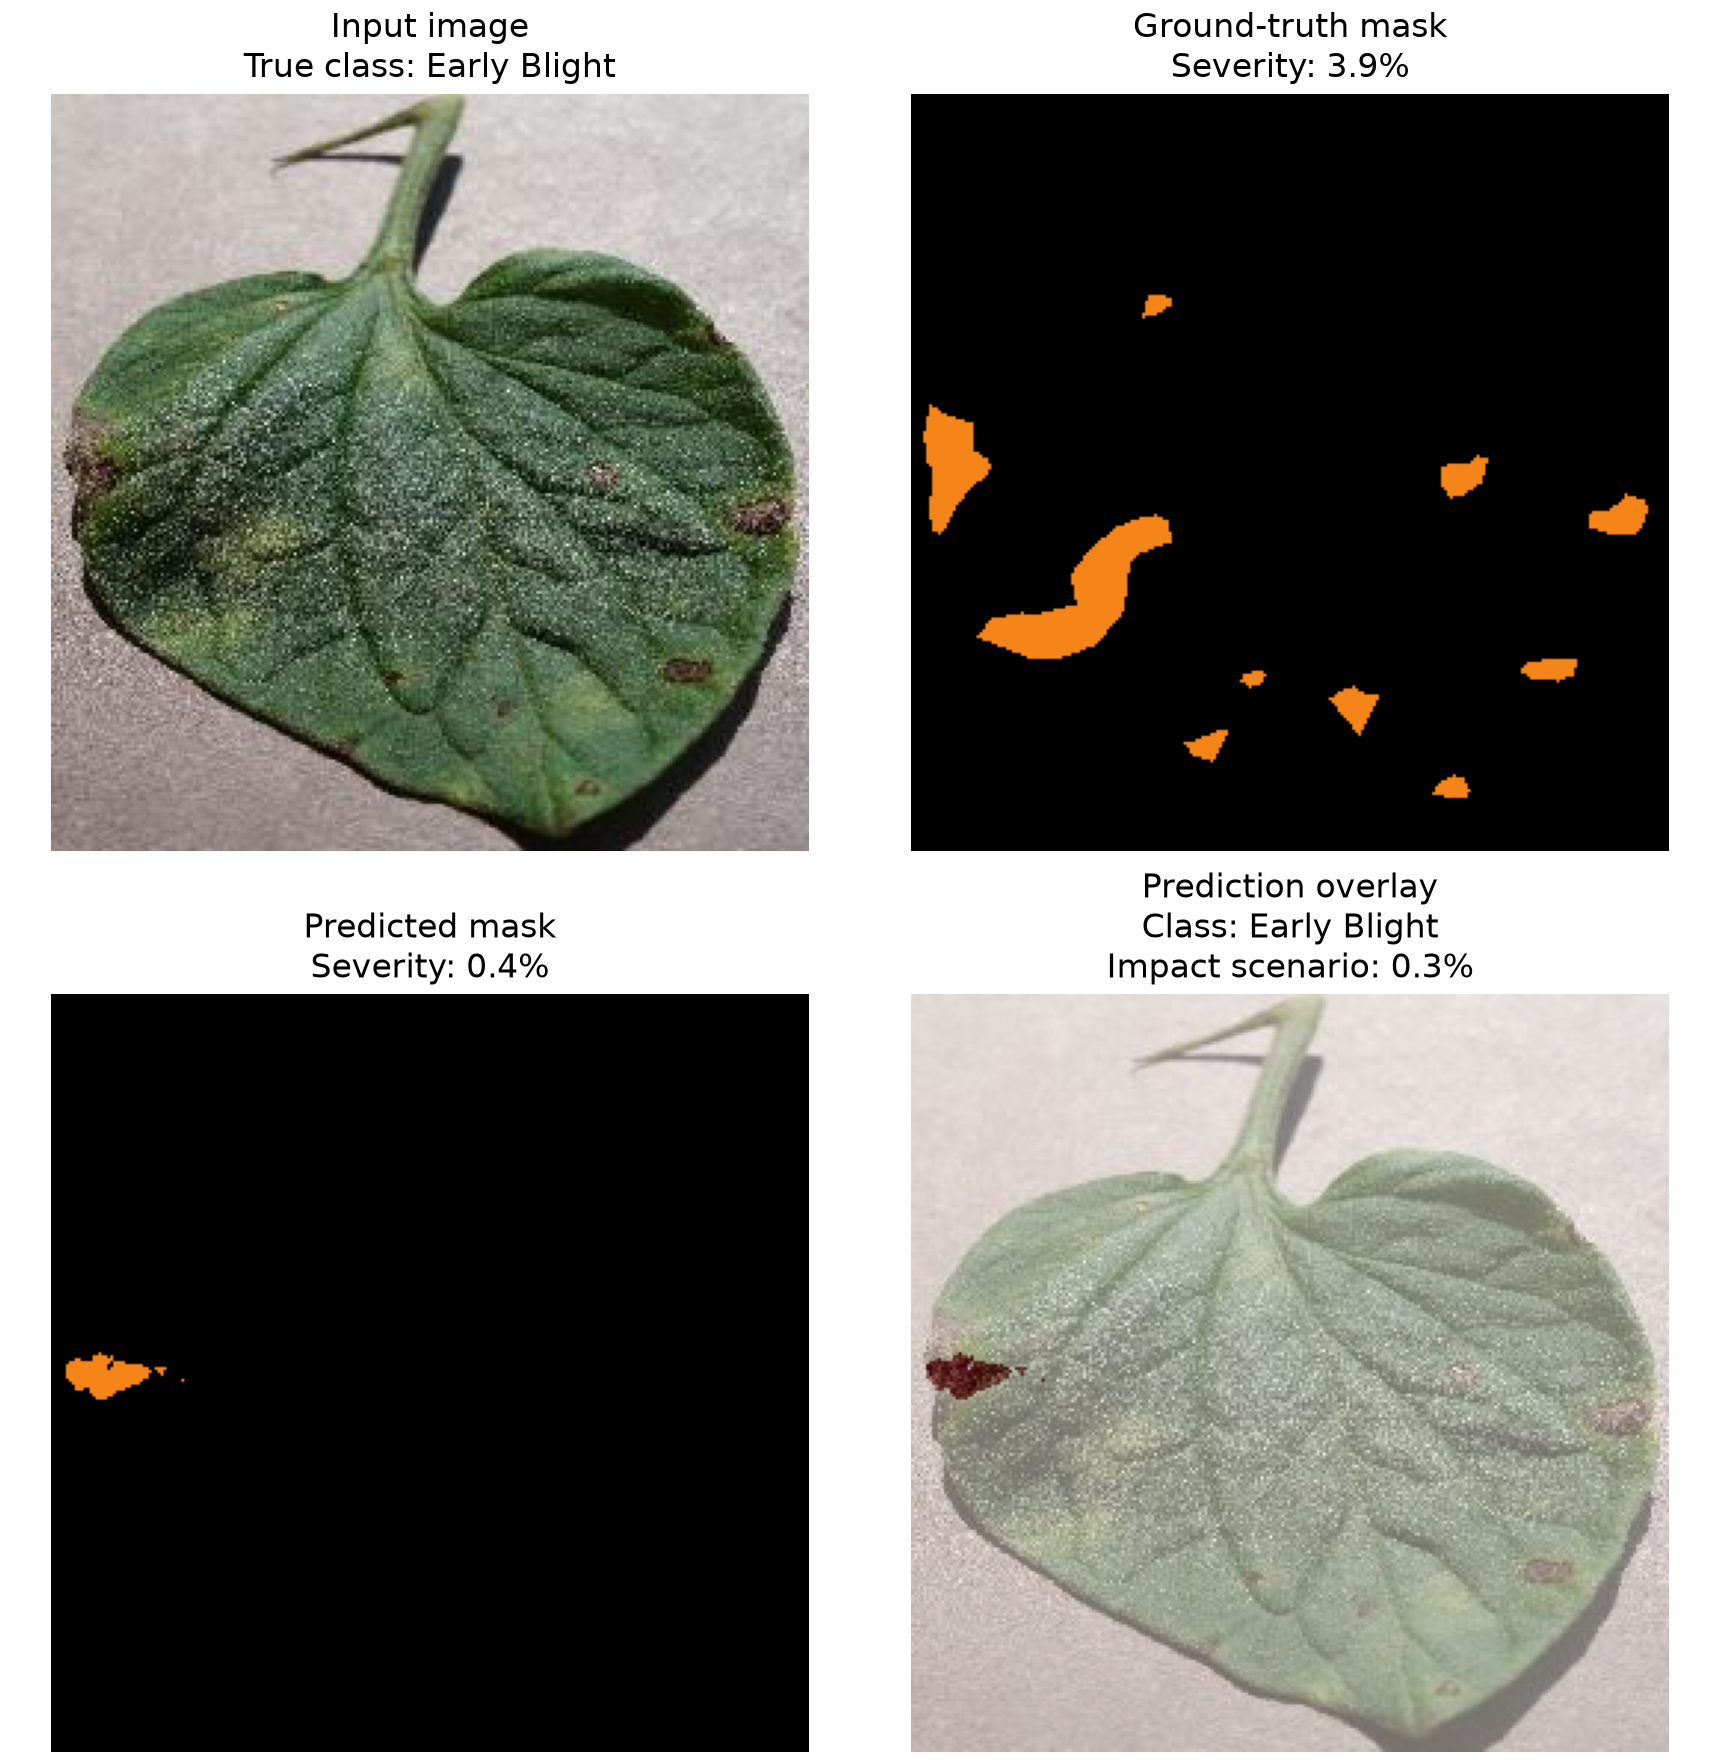
\includegraphics[width=0.94\textwidth]{mcunet-early.png}
  \caption{MCUNet-Seg prediction for an Early Blight sample.}
  \label{fig:mcunet-early}
\end{figure}

\paragraph{Figure analysis.}
Figure~\ref{fig:mcunet-early} shows strong under-segmentation of small Early Blight
spots. This visual result agrees with the low Early Blight recall of 0.2141.

\subsection{Model Complexity Results}
MCUNet-Seg reached its design goal of a small parameter count and low operation count.

\begin{table}[H]
\centering
\caption{Model parameter count and approximate operation count.}
\label{tab:efficiency}
\small
\begin{tabular}{lrr}
\toprule
Model & Parameters (million) & FLOPs (billion)\\
\midrule
DenseNet baseline & 6.96 & 5.67\\
DenseNet + attention & 26.10 & 7.54\\
Attention-Residual U-Net & 2.10 & 7.49\\
MCUNet-Seg & 0.73 & 1.86\\
\bottomrule
\end{tabular}
\end{table}

MCUNet-Seg used 65.2\% fewer parameters and about 75.2\% fewer approximate FLOPs than
the segmentation baseline. This makes it useful for future optimization, but the current
accuracy loss is too large for it to replace the
baseline when mask quality is the first priority.

\subsection{Severity and Yield-Impact Results}
On the 68 segmentation test images, the mean true severity proxy was 12.24\%. The
Attention-Residual U-Net predicted 9.43\% on average, with a mean signed error of
$-2.81$ percentage points. MCUNet-Seg predicted 8.14\% on average, with a mean signed
error of $-4.10$ points. This agrees with its low Early Blight recall.

For the segmentation baseline, the mean central potential impact scenario was 6.41\%.
The mean low and high scenarios were 5.46\% and 7.19\%. These numbers describe the test
images only. They are not measured farm-yield losses.

\subsubsection{Interpretation of Disease Effects}
The predicted impact values should be interpreted as an image-based risk indicator. A
higher lesion ratio increases the scenario value because more visible leaf area is
affected, but a single image cannot observe flowering, fruit set, fruit size, plant age,
or disease progression. The field evidence from TLCV is consistent with this interpretation:
the reported effects extended beyond leaf symptoms to plant height, fruit number, fruit
weight, and yield \cite{iftikhar2021tlcv}. It also showed that planting time, temperature,
and vector pressure changed disease incidence. Consequently, the model can quantify
visible disease burden and produce a transparent potential-impact range, but it cannot
claim that the range is the actual harvest loss for a plant or a field.

This interpretation is directly connected to the measured model results. DenseNet-121
classified the controlled test images with a macro F1 of 1.0000, so disease identity was
reliably separated within this split. The segmentation baseline reached 73.46\% macro
Dice, while MCUNet-Seg reached 52.44\%. Therefore, the impact estimate is more dependent
on segmentation quality than on classification quality in this experiment: an incorrect
lesion area changes $S$, and $S$ changes all three impact scenarios. The lower MCUNet-Seg
Dice score should consequently be read as greater uncertainty in its severity and
potential-impact outputs, even when the predicted disease label is correct.

\begin{figure}[H]
  \centering
  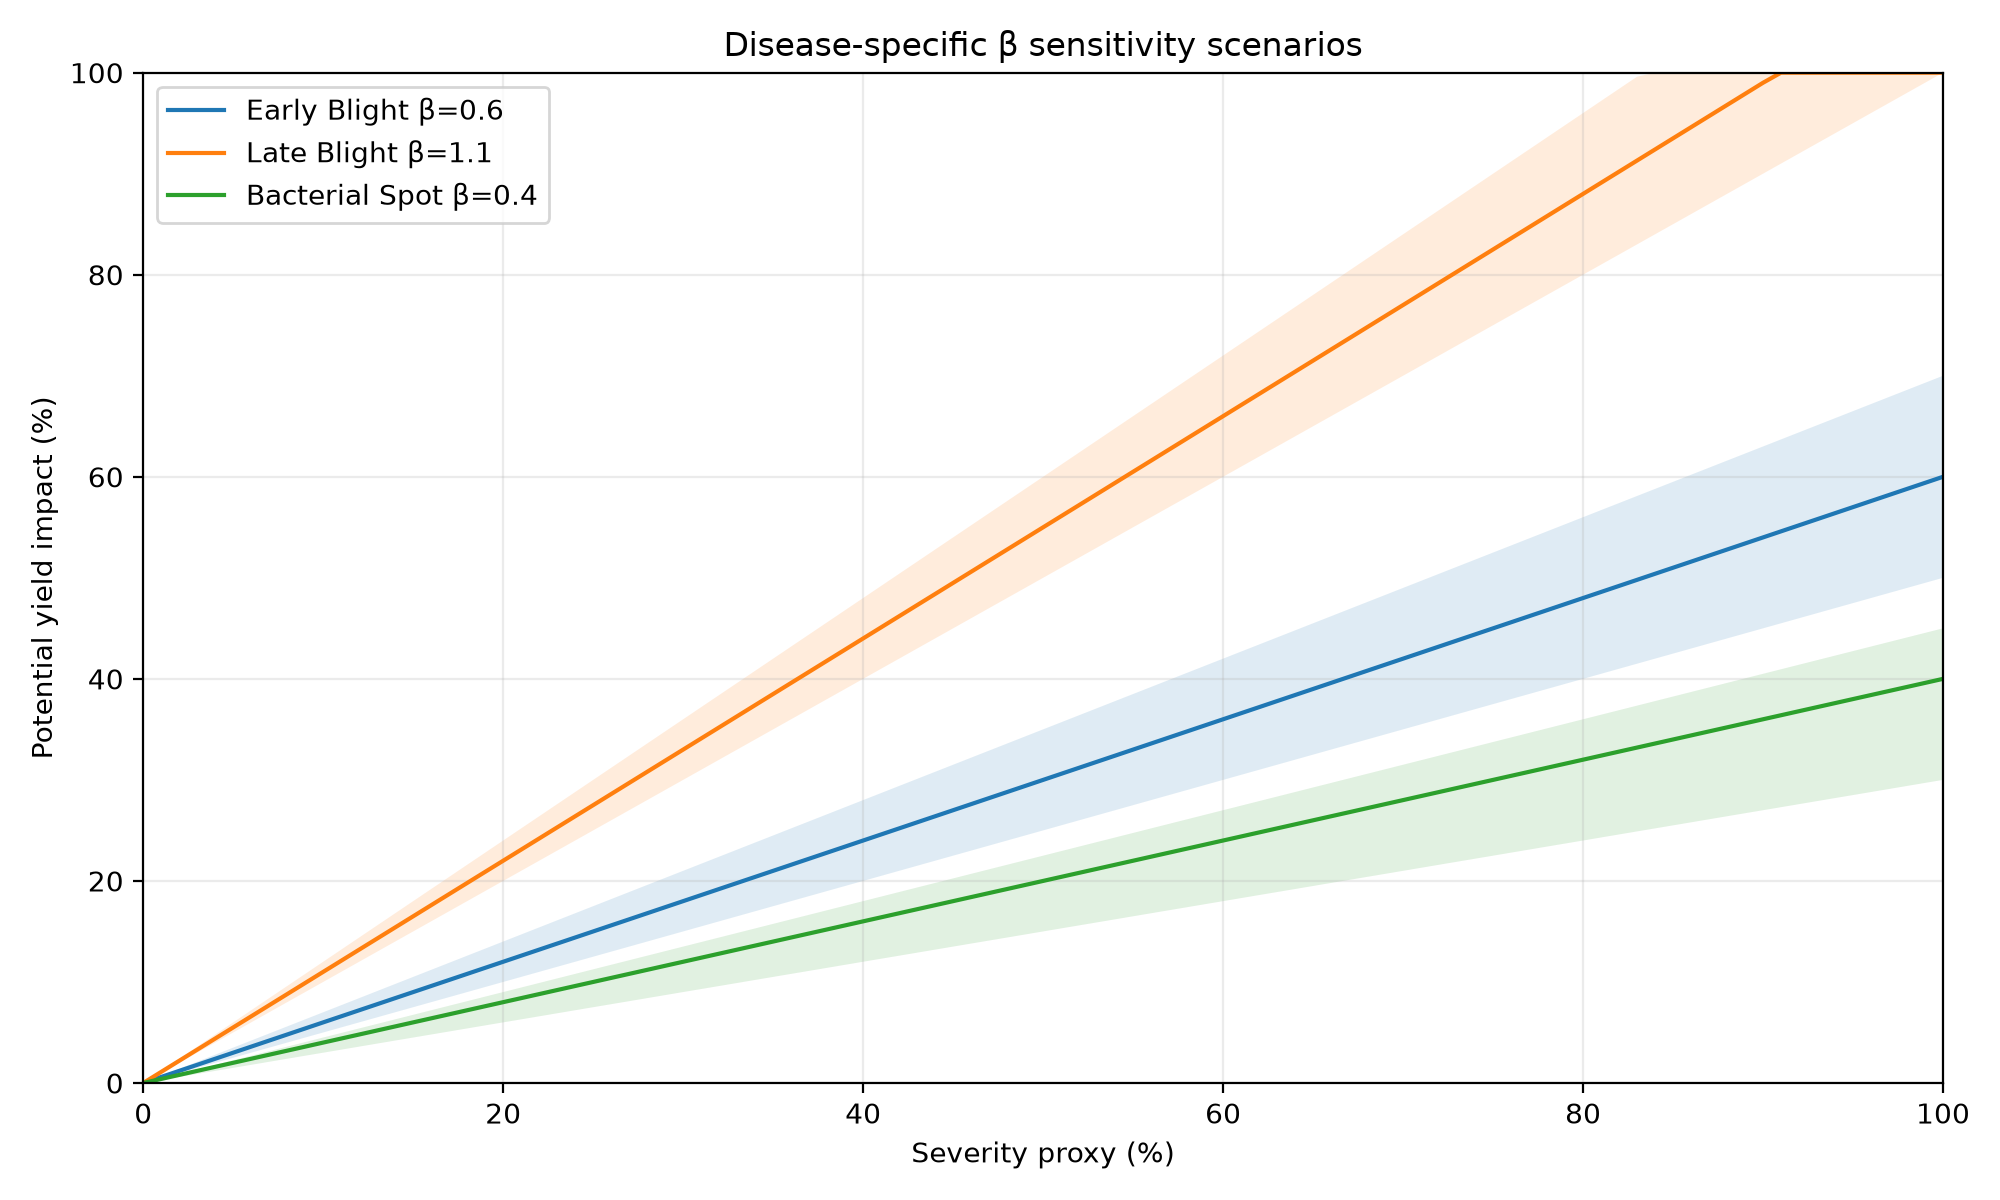
\includegraphics[width=0.98\textwidth]{yield-sensitivity.png}
  \caption{Low, central, and high beta sensitivity across severity values.}
  \label{fig:yield-sensitivity}
\end{figure}

\paragraph{Figure analysis.}
Figure~\ref{fig:yield-sensitivity} shows that Late Blight has the steepest assumed range.
The distance between low and high lines grows with severity. This makes the uncertainty
visible and is safer than reporting one exact percentage as a measured crop loss.

\subsection{Explainability Example}
Figure~\ref{fig:ig} shows one Integrated Gradients example from the held-out classification
set. The attribution map gives a qualitative view of the pixels that affect the predicted
class. It is useful for error review, but it is not a lesion annotation.

\begin{figure}[H]
  \centering
  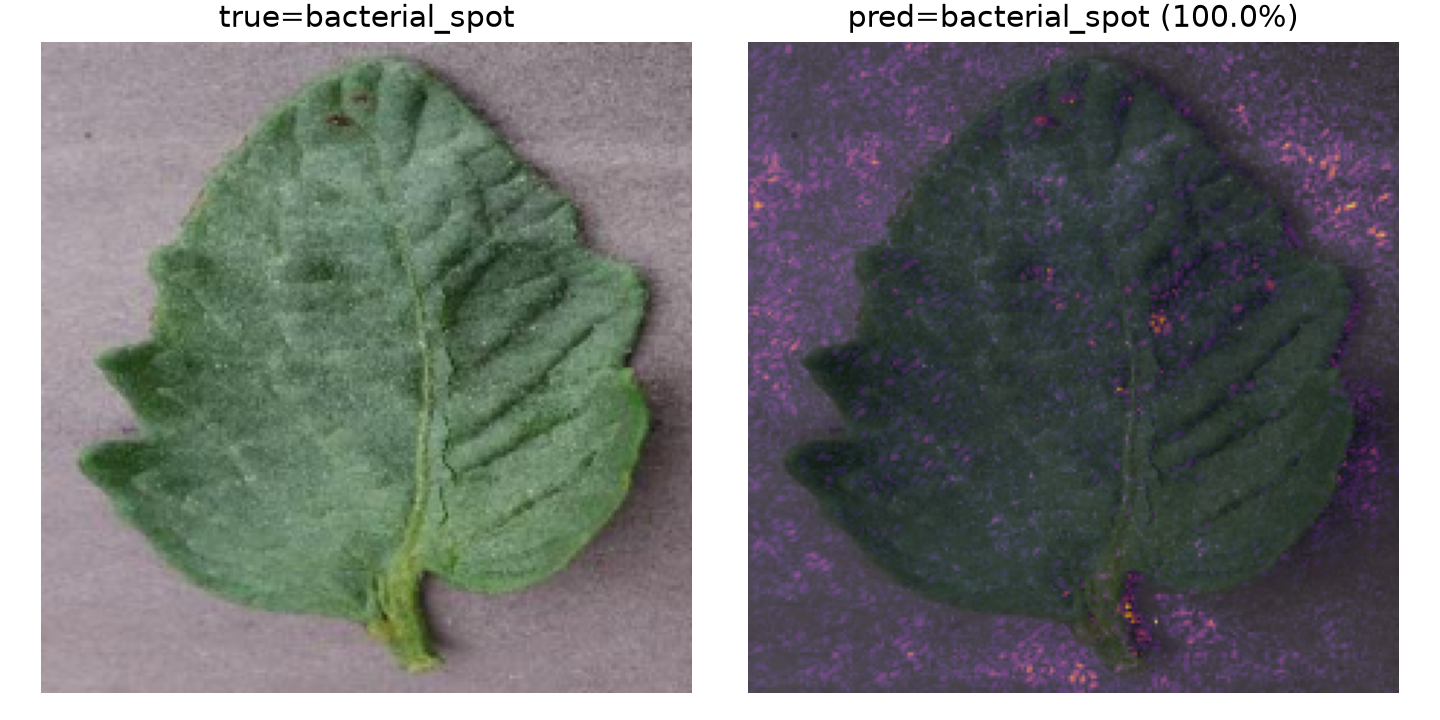
\includegraphics[width=0.98\textwidth]{integrated-gradients-example.png}
  \caption{Integrated Gradients explanation for a Bacterial Spot classification example.}
  \label{fig:ig}
\end{figure}

\paragraph{Figure analysis.}
Figure~\ref{fig:ig} shows where input pixels influenced one Bacterial Spot prediction. The
map gives useful visual evidence for model review. It does not prove that every highlighted
pixel is a lesion, so the semantic mask remains the source for severity.

% =============================================================================
\section{Experimental Setup}

\subsection{Software Environment}
The experiments were implemented in Python with PyTorch and torchvision
\cite{paszke2019pytorch}. OpenCV was used for image processing, while scikit-learn and
matplotlib supported statistical evaluation and visual analysis. The same dependency
versions and random seed were used for all model comparisons.

\subsection{Experimental Procedure}
Before training, an automatic data-quality gate checked image readability, label validity,
mask values, group separation, and split isolation. Four experiments were then executed in
a fixed order: DenseNet-121, the residual-attention classifier, Attention-Residual U-Net,
and MCUNet-Seg. Training history, model checkpoints, test predictions, per-class metrics,
confusion matrices, curves, and qualitative examples were retained for analysis.

Each interrupted experiment could continue from its latest training state. The stored
state included the model, optimizer, learning-rate scheduler, mixed-precision scaler,
early-stopping status, metric history, and random-number states. This procedure reduced
the risk of changing the experiment after an interruption and supported reproducibility.

\subsection{Final Evaluation Procedure}
Model selection used only the validation subset. After training, the checkpoint with the
best validation metric was evaluated once on the held-out test subset. Classification and
segmentation predictions were then combined to estimate severity and the three potential
yield-impact scenarios. All quantitative tables and qualitative figures in the Results
section were produced from this fixed evaluation procedure.

% =============================================================================
\section{Discussion}

\subsection{Main Findings}
The first finding is that the simple DenseNet-121 baseline was already strong enough for
the controlled classification split. Adding a large attention head increased model
complexity but reduced test macro F1 from 1.0000 to 0.9895. This answers the
first research question: the custom head did not improve this experiment.

The second finding is that the small segmentation model did not match the stronger
baseline. MCUNet-Seg reduced parameter count and FLOPs, but its Early Blight recall was
very low. The Attention-Residual U-Net is the better choice when segmentation accuracy is
more important than compact size.

\subsection{Why Classification Is Much Easier}
The classification set has 6,613 images, while the segmentation set has only 750 images.
Classification also needs only one image label. Segmentation must predict 65,536 pixel
labels for each 256$\times$256 image. Small lesions create a class-imbalance problem at
pixel level even when the number of images per disease is balanced.

PlantVillage backgrounds also make classification easier. The nearly perfect test result
may include visual clues that are stable in this controlled dataset but not in a farm image.
A cross-domain field test is needed before a real deployment claim.

\subsection{Important Limitations}
The largest limitation is the absence of paired field-yield data. The system does not see
plant-level disease progress, weather, cultivar, treatment, or final harvest. The output is
therefore a sensitivity scenario, not a causal yield forecast.

The leaf denominator is also heuristic. Some controlled images use almost the full frame
as the leaf region. This can underestimate or overestimate leaf-relative severity. Reviewed
leaf masks are needed for a stronger severity claim.

The yield-impact layer is also limited by biological transfer. The TLCV field study used
repeated observations, a defined cultivar, environmental exposure, vector pressure, and
direct measurements of fruit and yield \cite{iftikhar2021tlcv}. The present dataset does
not contain these paired variables and does not contain TLCV labels. Its impact values are
therefore scenario estimates that are informed by plant-disease literature, not causal
estimates of crop loss.

The segmentation test split contains only 68 images. Per-disease results can change with a
larger external test. The 750 masks also come from controlled leaf images. Field leaves can
have complex backgrounds, shadows, overlap, insects, and more than one disease.

Finally, this report describes one fixed seed. The split is deterministic and the run is
reproducible, but repeated seeds would provide confidence intervals for model comparison.

\subsection{Future Work}
The first next step is to collect field images with reviewed leaf and lesion masks. The
second is to collect repeated disease severity and marketable yield for the same plants.
This would allow the beta relation to be fitted and tested instead of assumed.

A suitable field protocol should record disease incidence, leaf-level severity, plant age,
cultivar, planting date, temperature, vector pressure, fruit number, fruit weight, and
marketable yield. The TLCV study illustrates why these variables are useful: incidence
changed across observation dates and planting dates, while fruit number, fruit weight, and
yield changed at the same time \cite{iftikhar2021tlcv}. Similar longitudinal records for
Early Blight, Late Blight, and Bacterial Spot would make the proposed impact layer more
specific and scientifically testable.

For classification, future work should test the baseline on PlantDoc or a local field set.
For segmentation, the Attention-Residual U-Net can be improved with stronger but safe
augmentation, multi-scale features, and a loss that gives more weight to small lesion
boundaries. MCUNet-Seg needs focused work on Early Blight recall. Knowledge distillation
from the stronger baseline may help keep the small model while improving masks.

Future work should also extend the system from a single-leaf image to a complete tomato
plant. An instance-detection or instance-segmentation model could first identify every
visible leaf and separate overlapping leaves. The current classification and lesion
segmentation stages could then process each detected leaf. Leaf-level severity values could
be combined to estimate the affected-leaf ratio and overall visible disease burden of one
plant. This plant-level measurement would be more useful for field monitoring, but it would
require images annotated with individual leaf boundaries, occlusion status, and repeated
observations during plant growth.

A final deployment study should test model export and quantization together with
accuracy on the real target platform.

% =============================================================================
\section{Conclusion}
This thesis built a complete pipeline for tomato leaf disease classification, lesion
segmentation, severity estimation, and potential yield-impact sensitivity analysis. The
pipeline supports healthy leaves, Early Blight, Late Blight, and Bacterial Spot, while Leaf
Mold is outside the project scope.

The real experiment showed that simple baselines were strong. DenseNet-121 reached
100.00\% macro F1 on the controlled classification test, while the custom attention model
reached 98.95\%. Attention-Residual U-Net reached 73.46\% macro Dice and clearly
outperformed MCUNet-Seg at 52.44\%. MCUNet-Seg was smaller and used fewer operations,
but the current loss in mask quality was large.

The common data splits, fixed seed, automatic state recovery, and consistent evaluation
policy also support reproducibility across the four experiments.

The yield part is intentionally limited. It provides transparent low, central, and high
scenarios based on lesion severity and disease type. A future field dataset with repeated
severity and measured harvest is required before the system can make a validated farm-yield
prediction.

% =============================================================================
\clearpage
\addcontentsline{toc}{section}{REFERENCES}
\bibliographystyle{plain}
\bibliography{references}

\end{document}
